\documentclass[a4paper,twoside,12pt]{book}
\usepackage[utf8]{inputenc}
\usepackage{listings}
\usepackage{amsmath}
\usepackage{amsthm}
\usepackage{amsfonts}
\usepackage{amssymb}
\usepackage[english]{babel}
\usepackage[a4paper]{geometry}
\usepackage{graphicx}
\usepackage{color,psfrag}
\usepackage{fancyhdr}
\usepackage{makeidx}
\usepackage{mathpazo}
\usepackage{mathrsfs}
\usepackage{float}
\usepackage{datetime}
\usepackage{titlesec}
\usepackage{datetime}
\usepackage{afterpage}
\usepackage{pdflscape}
\usepackage{ragged2e}
\sloppy

%\usepackage{hyperref}
%\usepackage[numbers]{natbib}
\usepackage[labelfont=bf,textfont=it,labelsep=period,width=\textwidth]{caption}
\usepackage[unicode,pdfstartview={XYZ null null 1},pdfview={XYZ null null 1},pdfpagemode=UseOutlines]{hyperref}
\usepackage{booktabs}
\usepackage{graphicx}
\newcommand{\ra}[1]{\renewcommand{\arraystretch}{#1}}
\newcommand\blankpage{%
    \null
    \thispagestyle{empty}%
    \addtocounter{page}{-1}%
    \newpage}
\newdateformat{monthyeardate}{%
  \monthname[\THEMONTH], \THEYEAR}


%szï¿œnek
\definecolor{szin}{rgb}{0.679,0.19,0.21}
\definecolor{szin2}{rgb}{0,0.445,0.734}
\definecolor{szin3}{rgb}{0,0.5,0}

\makeatletter
\let\stdl@chapter\l@chapter
\renewcommand*{\l@chapter}[2]{%
  \stdl@chapter{\textcolor{szin}{#1}}{\textcolor{szin}{#2}}}
\makeatother

%fejlï¿œc
\pagestyle{fancy}
\setlength{\headheight}{15.71667pt}
\lhead{\nouppercase{\rightmark}}
%\rhead{\nouppercase{\leftmark}}
\fancyhead[LE,RO]{\thepage}
\fancyfoot{}

%margomï¿œretek
\setlength{\marginparwidth}{0pt}
\setlength{\marginparsep}{0pt}
\setlength{\marginparpush}{0pt}
\setlength{\oddsidemargin}{24.1pt}
\setlength{\evensidemargin}{1pt}
\setlength{\footskip}{20pt}
\setlength{\headheight}{25pt}

    
%chapterstyles
\newcommand{\PreContentTitleFormat}{\titleformat{\chapter}[display]{\scshape\Large}
{\Large\filleft\MakeUppercase{\chaptertitlename} \Huge\thechapter}
{1ex}
{}
[\vspace{1ex}\titlerule]}
\newcommand{\ContentTitleFormat}{\titleformat{\chapter}[display]{\scshape\color{black}\huge}
{\color{szin}\Large\filleft\MakeUppercase{\chaptertitlename} \Huge\thechapter}
{1ex}
{\titlerule\vspace{1ex}\filright}
[\vspace{1ex}\titlerule]}
\newcommand{\PostContentTitleFormat}{\PreContentTitleFormat}
\PreContentTitleFormat


\begin{document}

\begin{titlepage}
\begin{center}

\textbf{\LARGE{Networks and Cities}}\\[3.3cm]


\includegraphics[width=3.45cm,height=2.3cm]{images/ceulogo.eps}\\[3.4cm]
{\Large{\textbf{Luis Guillermo Natera Orozco}}}\\[0.4cm]

\medskip

Department of Network and Data Science \\
Central European University\\ [1.2cm]

Supervisor: Federico Battiston \\
External Supervisor: Michael Szell

\vfill  

A Dissertation Submitted in Partial Fulfillment of the Requirements\\ for the Degree of Doctor of Philosophy in Network Science\\[2cm]

%
\includegraphics[width=3cm,height=2cm]{images/ceulogo.eps}\\[0.5cm]
% Central European University\\
% Budapest, Hungary

\vspace{1.0cm}
\the\year
\end{center}
\end{titlepage}

\newpage

\pagestyle{empty}

\mbox{}

\vfill

\noindent Luis Guillermo Natera Orozco: \emph{Networks and Cities}, \copyright \\
\the\year \\ All rights reserved.



\mbox{}

\pagestyle{empty}

\newpage


\chapter*{Researcher declaration}
I Luis Guillermo Natera Orozco certify that I am the author of the work Networks and Cities. I certify that this is solely my own original work, other than where I have clearly indicated, in this declaration and in the thesis, the contributions of others. The thesis contains no materials accepted for any other degrees in any other institutions.  The copyright of this work rests with its author. Quotation from it is permitted, provided that full acknowledgement is made. This work may not be reproduced without my prior written consent. 

\subsection*{Statement of inclusion of joint work}
%I confirm that Chapter 3 is based on a paper which was written in collaboration with Taha Yasseri, Bal\'azs Lengyel, and J\'anos Kert\'esz. I conceived of the idea to relate social capital with local corruption risk outcomes by comparing data from procurement contracts and the online social network. Dr. Kert\'esz and I conceived the details of the implementation. Dr. Lengyel and I collected data on municipalities. Dr. Yasseri and I developed the methods used. I carried out the analyses of the data. All authors contributed to the writing of the paper on which the chapter is based and gave final approval for publication. Dr. Kert\'esz endorses this statement with his signature below.

\vspace{.2cm}

%I confirm that Chapter 4 reuses a plot from a working paper written in collaboration with Mih\'aly Fazekas on the impact of corruption on public procurement market structure. The plot, which I drafted, serves as a prototypical example of the representation of procurement markets as networks. The remaining contents of the paper are independent of the contents of Chapter 4. Dr. Fazekas endorses this statement with his signature below.


\vspace{.2cm}

\noindent
%I confirm that Chapter 5 is based on a working paper which was written in collaboration with J\'anos Kert\'esz. I conceived of the idea to use a co-bidding network framework to study collusion. Dr. Kert\'esz and I collaborated on developing and improving the methods used in the paper. I collected the datasets used and implemented the methods. Dr. Kert\'esz and I and both contributed to the writing of the paper on which the chapter is based and gave final approval for submission. Dr. Kert\'esz endorses this statement with his signature below.



\vspace{0.5cm}
\noindent
Signature of PhD Candidate:

\vspace{2cm}
\noindent
\monthyeardate\today


\vspace{3.5cm}
\noindent
Signature of Dr. Federico Battiston, endorsing statement of joint work:

\vspace{2cm}
\noindent
\monthyeardate\today


\vspace{3.5cm}
\noindent
Signature of Dr. Michael Szell, endorsing statement of joint work:

\vspace{2cm}
\noindent
\monthyeardate\today

\vspace{3.5cm}
\noindent
Signature of Dr. Orsyola V\'as\'arhelyi , endorsing statement of joint work:

\vspace{2cm}
\noindent
\monthyeardate\today




\chapter*{Abstract}
%Though corruption is a broad notion encompassing many kinds of behavior, it always has a relational aspect. Consider how a driver bribes a policeman, how a minister steers a contract to build a hospital to his son-in-law's construction company, how two managers from different firms agree to avoid competition in a region, or how a regulator goes easy on a potential future employer during an audit. The observation that interactions between people, firms, and institutions are where corruption happens is not a new one, but certainly merits further investigation. A better understanding of the relationship between the networks that these connections form and corruption can explain why corruption is so difficult to defeat.

%This thesis applies the methods of network science to the study of corruption and its relationship with markets and society. I argue that corruption emerges from specific patterns of interactions that can productively be described using networks. The dyads of actors engaging in a corrupt behavior, the driver and policeman, minister and son-in-law, etc., are embedded in networks of social relations that facilitate corruption. Within this framework, the thesis addresses several questions about corruption. Why does corruption persist in certain communities? How does corruption relate to the organization of markets? How does corruption emerge when it depends on cooperation in highly adverse circumstances? I address these questions empirically using newly available micro-level data on corruption risks in public procurement.

%Starting with a study of Hungarian towns, I relate corruption risk in local government contracts to the structure of their social networks. I find that fragmented towns have higher corruption risk, while towns with residents that have diverse connections have less. This suggests that corruption is embedded in the social networks of places. Next I zoom out to the national level, comparing the procurement markets, conceptualized as networks of issuers and winners, of different EU countries. I find a strong relationship between centralization and corruption risk. On the other hand, heterogeneity in market responses to changes in government across the EU suggests that corruption can be organized in many different ways. Finally, I investigate cartels, or groups of firms that illegally agree to avoid competition. By drawing networks of firms that bid for the same contracts I highlight niches in markets where cartels are more likely to thrive.


\thispagestyle{empty}

\chapter*{Acknowledgements}

% I would like to acknowledge several individuals who have, whether they realize it or not, significantly influenced this work. First I must thank my advisor J\'anos Kert\'esz for his continued support and confidence. His guidance has been invaluable and his patience is much appreciated.


\thispagestyle{empty}
% \textsc{
% \newpage
% \frontmatter

% \pagestyle{fancy}

% \newpage
% \addcontentsline{toc}{chapter}{Contents}

% \PreContentTitleFormat


% \tableofcontents

% \PreContentTitleFormat

% \newpage

% \PreContentTitleFormat

% \pagestyle{fancy}

% \newpage
% \PreContentTitleFormat
% \pagestyle{fancy}

% \listoftables
% \addcontentsline{toc}{chapter}{List of Tables}}

%\listoffigures
%\addcontentsline{toc}{chapter}{List of Figures}

% \PreContentTitleFormat
% \newpage
% \mainmatter
% \ContentTitleFormat

%\chapter{Introduction}

Corruption is a major cause of suffering around the world. It slows economic growth~\cite{mauro1995corruption}, stifles innovation~\cite{rodriguez2014quality}, and increases inequality~\cite{gupta2002does}. The social impacts of pervasive corruption in a society, reflected for example in distrust of government and strangers~\cite{rothstein2013corruption} and in the low quality in government services~\cite{lambsdorff2001corruption}, suggest that corruption reinforces itself in a kind of feedback loop. Feeling that society is rigged, individuals adapt to their circumstances and play by the local rules. Like many other social scientific problems, understanding the emergence or persistence of corruption is difficult because it manifests both in individuals and societies. 

This dichotomy is one reason why there are multiple definitions of corruption. The World Bank and Transparency International define corruption as ``the abuse of public or corporate office for private gain'' and ``the abuse of entrusted power for private gain,'' respectively~\cite{nye1967corruption,rose1978corruption,transparency2007global}. This definition provides a good benchmark to use when deciding whether an individual's behavior should be considered corrupt. Recently, scholars of government and institutions have focused on a more macro-oriented definition of good governance, namely: ``the degree to which the exercise of public authority follows the principle of universalism or impartiality''~\cite{rothstein2008quality}. The presence of partiality or particularism in the decision making of public actors is a useful definition of corruption because it defines a norm of behavior that can be applied to various contexts~\cite{mungiu2013controlling}.

These two perspectives have had some success in quantifying causes and effects of corruption, building measures of the prevalence of corruption in countries and regions, and proposing policy interventions to improve the control of corruption in society. They share several important core concepts, for example both reference corruption as a kind of behavior existing at the intersection of the public and private domains. Both refer to the exploitation of power or advantage, presumably to the detriment of a wider group of people.

The definition of corruption based on the lack of impartiality has become increasingly relevant as researchers of corruption focus on grand corruption, distinct from petty corruption. Corruption is deemed petty when it is impersonal and transactional - for example when someone bribes a driving instructor to pass an exam or a policeman to avoid a speeding ticket. Grand corruption refers to coordinated, organized behavior to siphon resources to specific groups or networks of people~\cite{Mungiu-pippidi2006,fazekas2016}. When examples of grand corruption are discovered they are typically front page headlines, as for example in the case of Petrobras, Brazil's state-owned petroleum company, whose executives were found to have taken nearly \$10 billion of bribes and kickbacks from a group of 16 large construction firms in exchange for awarding them overpriced contracts~\cite{watts2017operation,ribeiro2018dynamical}. Over 160 people were arrested and 93 convicted, including the former President of Brazil.

 Such a large conspiracy with such significant payoffs to its participants is only possible as a collective effort of many people. Despite having a larger target to aim at, it is difficult for authorities to combat grand corruption. This is because grand corruption is often organized in a sophisticated way, with its actors having specific responsibilities and roles, and connections organized in a way to limit their vulnerability as a whole~\cite{ferrali2018corruption}. Organized crime groups~\cite{calderoni2011strategic} and the September 11th hijackers~\cite{krebs2002mapping} structured themselves in a similar manner. Grand corruption is a difficult topic for academic research for these same reasons and also because it is unlikely that large conspiracies can be understood in terms of a sequence of ``abuses of public or corporate office for private gain''. Somehow such conspiracies are much more complex social outcomes than the sum of the individual behaviors of their members.
 
 Throughout this thesis when we speak about corruption, we will be referring to grand corruption and its organization, rather than instances of petty corruption. Though the prevalence of bribery and its acceptance in society are likely correlated with the prevalence of grand corruption, it is not essential to its functioning.

While framing corruption in terms of the norms and rules of society may be more applicable to the study of grand corruption than the transactional view of corruption focusing on bribery, it suggests an over-socialized description of corruption. In an extreme interpretation, the environment determines the actions of individuals, who merely ``internalize norms and seek [to conform] to the expectations of others''~\cite{wrong1961oversocialized} and so participate in corruption. Such a perspective not only fails to give a satisfying answer to the question of why certain places have developed a good control of corruption while others have not, but is also empirically unsupported. We will see that there is significant variation in the prevalence of corruption as we measure it within countries, even at the level of towns. It also has limited ability to explain how the prevalence of corruption in a place might change over time. Indeed, the Petrobras scandal offers some hope for Brazil: in the end powerful people were imprisoned for their corruption.

As they focus on individuals and societies, respectively, both definitions avoid mentioning that corruption, like nearly all socioeconomic activity, happens between actors. In this thesis we consider corruption as a networked phenomenon~\cite{granovetter1985economic}. It is a property of the interactions between groups of actors such as people, firms, institutions, which evolves as these interactions change. In his 1985 paper on the embeddedness of economic action in social structure, Mark Granovetter suggested that ``force and fraud are most efficiently pursued by teams, and the structure of these teams requires a level of internal trust--``honor among thieves''-- that usually follows preexisting lines of relationship.'' In other words, Granovetter is suggesting that particular social structures or networks are required to scale corruption to high levels. We do not discard the productive micro-level definitions of corruption by the World Bank or Mungiu-Pippidi, but we do change the way they are applied.


We will demonstrate that this approach can describe in novel ways the organization and roots of corruption at various scales from towns to nations. It complements micro and macro-level frames of corruption by considering what happens in between.

Theory aside, why might networks be a useful in the study of corruption, for example in its measurement, detection, or diagnosis? Grand corruption, as its name suggests, requires organization and coordination. Such organization may manifest explicitly as a social network of specific actors, say members of parliament and heads of firms. It should also leave fingerprints in the interactions between firms and institutions doing business and exchanging money. Crucially, several recent developments make it possible to examine empirically the relationship between corruption and the networks of actors. The growth of the internet and its use by governments has created a wealth of fine-grained administrative data on interactions between the public and private sectors. 

One distinguished example of such data is information on public contracting or procurement markets, which accounts for upwards of 20\% of GDP in OECD countries~\cite{oecdprocurement}. Recently, researchers have developed ways to measure corruption risk in the award of such contracts~\cite{fazekas2016corruption,fazekas2017uncovering}. This data and measurement approach provides us with the micro-level data to undertake a network-based analysis of the phenomenon of corruption. We argue that this data, at present, offers the best possible approach to an evidence-based, data-driven anti-corruption research program as proposed by Mungiu-Pippidi in 2017~\cite{mungiu2017time}.

Nearly in parallel, researchers studying biological~\cite{alm2003biological}, ecological~\cite{ings2009ecological}, social~\cite{borgatti2018analyzing}, economic~\cite{schweitzer2009economic,jackson2010social}, and spatial ~\cite{barthelemy2011spatial} phenomena have made fundamental advances in their fields by using a network perspective. A by-product of these minor revolutions in different physical and social sciences is the emergence of set of tried and tested methods for studying networks within data. These efforts extend the pioneering work of sociologists and anthropologists~\cite{moreno1941foundations,freeman1978centrality,wasserman1994social}, who have been working on social networks since the 1940s, to new contexts and larger scales\footnote{For an excellent history of research on social networks we refer the reader to the review of Freeman~\cite{freeman1996some}. For an overview of the current relationships between the different traditions of network analysis, we refer the reader to Hidalgo's review~\cite{hidalgo2016disconnected}.}. This recent work on networks forms an emerging field of research called network science, which has created a rich tool set for the study of complex systems.


This thesis proposes to leverage these developments to extend the state of the art in corruption research. Specifically, we claim that corruption risk can effectively be measured at the micro-level using administrative public contracting data, and that by using network science methods we can describe the organization or structure of corruption. We do this in three contexts: relating social networks and corruption outcomes of towns, describing the relationship between corruption risk and market structures at the scale of countries, and analyzing the emergence of illegal cartel behavior among firms. In all three chapters we provide both a theoretical contribution to the understanding of corruption and policy implications. 

First we describe how the structure of social networks are related with the prevalence of corruption in local government contracting using data from Hungarian settlements. By linking social structure with corruption we strengthen our claim that corruption is in general a networked phenomenon. 

Next we zoom out to the level European countries, mapping their procurement markets as bipartite networks of public institutions and the firms they contract with. These networks have rich structure related to their level of corruption risk. By observing how corruption risk is distributed in these networks and how actors with high risk scores respond to political shocks, we highlight novel distinctions between the organization of corruption in different countries. Among EU countries we find significant heterogeneities, for example that in some countries corruption risk is concentrated in the core of the procurement markets, while in others it is more common in the periphery. 

Finally, we shift focus to cartels in procurement markets, transferring the perspective we have developed to study corruption to a different but related economic problem. Cartels are groups of firms which illegally avoid competition to maximize their profits. We propose a framework to map markets of competing firms using contracting data, to identify groups of frequently interacting firms, and to measure their potential for forming cartels. 

The remainder of the thesis is structured as follows:
\begin{itemize}
\item Chapter 2: Here we review past work on the conceptualization and measurement of corruption, introducing measures based on both perceptions and administrative data and comparing them. We also review the literature on network aspects of corruption.
\item Chapter 3: In this chapter we relate the social networks of Hungarian towns using data from an online social media portal with the amount of corruption risk in their local governments.
\item Chapter 4: In this chapter we quantify corruption at the national level using data on public contracts awarded by member states of the European Union. By mapping procurement markets as networks, we can examine the distribution of corruption risk in different countries, and observe how they react to political shocks.
\item Chapter 5: In this chapter we apply network methods to the problem of cartels, transferring the principles developed in earlier chapters to a domain adjacent to corruption. We consider the emergence of illegal cooperation among firms in procurement markets using records of their bidding behavior. We observe a ``hot spots'' in the network topology where collusion appears much more sustainable.
\end{itemize}

We conclude by tying our findings together, presenting some of their diagnostic interpretations, and suggesting future avenues of research.\pagestyle{fancy} %Introduction
%\chapter{Related Work}

In this chapter we discuss relevant previous work on corruption, including its measurement and its relational aspects, in order to orient the thesis. Following a brief survey of classical studies of corruption, we review how corruption is studied using experiments and models. These results give us insights into how corruption functions at smaller scales and suggests potential mechanisms to investigate. Next comes a review of how corruption is measured, considering surveys, and indicators derived from administrative data. We then survey findings on the causes and consequences of corruption, noting how corruption is measured in each result. With these results in mind, we argue that measuring corruption using indicators derived from administrative data is the most promising way to study the organization and structure of corruption because of its granularity. Correlations between such indicators and other measures of corruption demonstrate the validity of our chosen approach. Finally, we review applications of network methods to the study of corruption and crime more generally.

As suggested in the introduction of this thesis, corruption is a long-studied topic of interest to many branches of the social sciences. The result is that corruption has been studied from a variety of viewpoints, reflecting broad trends in how different fields have productively conceptualized human behavior at various times~\cite{elster2015explaining}. Before reviewing the most recent theoretical and empirical approaches to the study of corruption, we briefly highlight two such viewpoints, framing them as micro- and macro- oriented perspectives. 

A major \textit{micro-}oriented perspective on the study of corruption is the principal-agent framework~\cite{klitgaard1988controlling}. In this framework, the principal represents an actor in charge of monitoring agents, seeking to block or limit corruption, referring sometimes to a high-level policymaker or to the public as a whole. The agents are individual bureaucrats, citizens, or politicians who weigh incentives to engage in corruption or to follow the rules. In a seminal work on this framework Klitgaard~\cite{klitgaard1988controlling} describes corruption with a formula at the agent level: "corruption equals monopoly plus discretion minus accountability". Schleifer and Vishny~\cite{shleifer1993corruption} model the decision of bureaucrats to take bribes as a cost-benefit analysis of rational agents. 

The results of such models offer immediate policy recommendations, for instance to increase accountability when an agent occupies a monopoly position. More generally speaking, this approach to corruption emphasizes necessary conditions for the control of corruption, for instance the existence of constraints in policy-making. It falls short in describing sufficient conditions for effective control of corruption. The principal-agent framework suffers from several flaws, such as the assumption that a clean principal exists or can be created (for example by establishing an anti-corruption agency), or that marginal changes to incentives can change a thoroughly corrupt equilibrium~\cite{persson2013anticorruption}. Mungiu-Pippidi and Dadasov suggest that a principal-agent framework is only useful when ``corruption is an exception and the broader norm is ethical universalism.''~\cite{mungiu2016measuring} In other words, the principal-agent framework is an under-socialized approach to corruption, neglecting the norms and context that corrupt actions are embedded in.

Researchers adopting a \textit{macro-}orientation to the study of corruption often seek to compare and explain the differences in outcomes of countries using structural or institutional factors. Structural factors include the level of development or education, or the legacy of a country's history (for instance as a colony)~\cite{acemoglu2002reversal}. Work by Treisman, for instance, shows a significant positive relationship between how long as place has been democratic and its control of corruption~\cite{treisman2000causes}. In general wealthier countries with an education citizenry have less corruption~\cite{treisman2007have}. Institutional factors refer rather to the current legal organization of a place, for instance its constitution, and its politics. There is for example some evidence that political competition is an important ingredient to effective control of corruption~\cite{broms2017procurement}. Given, however, the heterogeneity of corruption outcomes at sub-national levels~\cite{charron2014regional}, there is a kind of natural resolution limit to entirely macro-based approaches to the study of corruption. We argue that such an approach suffers from an over-socialized perspective which struggles to explain how countries actually overcome corruption.

In the rest of this chapter we present previous experiments, models, and empirical studies that further demonstrate the potentially networked nature of corruption in a variety of contexts and at different scales. Again we emphasize that we do not discard the perspectives we describe above, but rather highlight how they can be enhanced by an alternative perspective.

 
\section{Experiments}

A major limitation of the social sciences has been the inherent difficulty of carrying out experiments to test hypotheses about the social world. In the natural sciences, experiments are a crucial ingredient of many research projects. Often, social scientists can only use observational data to test their ideas in the context of the social world. An alternative to using observational data is to test hypotheses about the social world in artificial or specific contexts. The former refers to laboratory experiments, in which participants are put into situations emulating the real world and their reactions to stimuli are observed~\cite{camerer2011advances}. Using computers and remote participation, the potential scale of such experiments has vastly increased, sometimes involving hundreds of simultaneous participants~\cite{arechar2018conducting}. The latter notion refers to randomized control trials, in which a sample of a population (of individuals, towns, regions) is split into treatment and control groups, an intervention is applied to the treatment group, and outcomes are tracked~\cite{duflo2007using}. Such methods offer convincing evidence of the effect of intervention, at great cost. Randomized control trials are expensive to implement and carry on over time. Both kinds of experiments have been applied to the study of corruption~\cite{abbink2006}.

Lab experiments have been used to test the hypothesis that corruption is a cultural phenomenon by having participants from different cultures play games in which there is economic incentive to cheat or behave in a corrupt manner. Cameron et al.~\cite{Cameron2009} find high cross-cultural variation (comparing subjects from Australia, India, Indonesia, and Singapore) in the propensity to punish corruption, and less variation in actually engaging in corruption. This finding suggests one reason why social networks may have an important role to play in corruption: actors across cultures may not be more or less willing to engage in corruption, but rather face different consequences depending on their alters. Other experiments show that when individuals are given opportunities to take corrupt actions without consequences in one round of a game, they are more likely to be dishonest when they are unsure about the consequences. This suggests that experience with corruption increases willingness to engage in corruption, again suggesting a role for networks in the spread of corruption~\cite{Shalvi2016,Gachter2016}.

A third example of the study of corruption in a laboratory environment dramatically underscores the collaborative nature of corruption~\cite{weisel2015collaborative}. Weisel and Shalvi have pairs of subjects play a six-sided dice rolling game. The first player rolls a die, observes its outcome privately, and reports it to his partner. The partner then rolls his die, also observing the outcome in private. The players are paid proportionally to the value of their roll if and only if both players \textit{report} having rolled the same number. In the results, both the frequency of matches and the frequency of high numbers (fives and sixes) reported by the players is many times greater than what would be expected if both players were honest. The amount of dishonest reporting is also significantly higher in this two player game than in a similar one player game. These results suggest that collaboration can facilitate dishonest behavior, perhaps via the diffusion of responsibility. On the other hand, the classic study of Kahneman, Knetsch and Thaler~\cite{kahneman1986fairness} suggests that individuals will reject unfair distributions at cost to themselves, so corrupt collaborations likely require a careful distribution of resources to be effective.

Despite their artificial nature, these experiments provide insights into potential underlying mechanisms of corruption. The studies we have highlighted suggest the importance of other people in an actor's choice to be corrupt. Others can be tolerant of corruption, they can provide examples, and they can even be accomplices. 

There are several notable large-scale field experiments relevant to our work. Most prominent is the work of Olken in Indonesian villages~\cite{olken2007monitoring}. Olken designed a series of interventions applied in a randomized way to over 600 villages that were about to start building roads using funds from a nationwide infrastructure project. A random sample of villages were informed that their implementation of the project would be audited by the central government, and that the results would be read publicly in an open forum in the village. This random intervention tests the effectiveness of top-down checks on corruption. Olken was also interested in the potential for bottom-up methods to combat corruption, so in another subset of the villages, he organized public accountability meetings with the project officials. Within this subset Olken ran another experiment: allowing residents of some villages to relay anonymous information about the project which would be read aloud at the meetings. These two interventions test the ability of grassroots organization to fight corruption. 

In order to measure corruption in the delivery of the road construction projects, Olken hired a team of engineers and surveyors who generated independent estimates of the costs of projects. Comparing these estimates on a line-item basis with the observed outcomes, Olken found that the roads built cost 27\% more on average than what the engineers estimated. Top-down auditing decreases the discrepancy between between cost and the independent estimates by nearly a third to 19\%. The bottom-up grassroots organizing had no significant effect on corruption. Following up with a household survey, Olken found that family members of local government officials were significantly more likely to have been employed on the road project in audited towns. This suggests that the guarantee of a top-down audit of expenditures had a substitution effect - instead of reporting higher prices and pocketing the difference, corrupt leaders hired their family members. Contrasted with the insignificance of the grassroots intervention, this final observation highlights the importance of distinguishing between different kinds of social connections when studying corruption.

Bertrand et al. provide a second example of the use of randomized control trials~\cite{bertrand2007obtaining} to study corruption. Participants in the study, run in India, are tasked with obtaining a driver's license. A third of the participants are offered a bonus if they obtain the license quickly, the second third are given free driving lessons, and a remaining third serve as a control. While members of both treated groups are more likely to obtain a license than members of the control group, members of the so-called bonus group accomplish this by paying bribes to third-party agents. These agents are a constant presence in Indian bureaucracy - nominally they are hired to stand in line on behalf of clients. 

Many of members of the bonus group obtain a license without taking an exam, and are found to have significantly worse driving skills in a surprise exam - a good example of an externality of corruption. The agents arranging the corrupt transfer play an interesting role: they insure that license seekers do not interact directly with bureaucrats in the extra-legal process. They are by definition brokers - the crucial network connections that facilitate corruption in this environment.

In some rare cases, governments carry out randomized audits of public works and records. The most notorious example comes from Brazil, where a 2003 federal government program introduced lottery-based audits of municipalities~\cite{ferraz2008exposing,mucco2017anti}. Researchers have used this data to quantify corruption at the municipal level in Brazil and to measure how corruption impacts incumbent electoral performance, and what impact local media have. A recent study shows that the electoral effects of revealed corruption spill over into neighboring towns ~\cite{mucco2016learn}. Voters in towns neighboring a corruption scandal will punish politicians of the same party as the neighboring mayor in their own election.  


Well-designed randomized control experiments can measure interesting causal relationships between variables relevant to corruption. However they do have some significant limitations. They are expensive and are difficult to scale. By definition they cannot compare effects in different contexts or environments unless the treatment itself is the difference. Randomized audits of public works seem to be cost-effective, as demonstrated by Olken's work in Indonesian villages and in the case of Brazilian municipalities, but we do not know an example of a central government body instituting random audits of its own actions at a large scale (consider for instance that corruption in Petrobras was going on at the same time as the introduction of the randomize audits of municipalities in Brazil). 

\section{Models}

Purely abstract models of social systems can provide useful ideas to researchers of social phenomena~\cite{miller2009complex}. In this section we describe some previous work on corruption which applies abstract models or agent-based simulations. Economic Nobel Laureate Jean Tirole created a model of the persistence of collective reputation to suggest that once bad behavior becomes a structural phenomenon, it is difficult to get rid of~\cite{Tirole1996}, echoing the experimental work cited above. Lambsdorff~\cite{Lambsdorff2002} points out that the informal mechanisms used to enforce corrupt agreements and notion of mutually-assured-destruction lock partners in corrupt deals together. Ferrali~\cite{ferrali2018corruption} models the spread of corruption as a game played on a network, finding that modular networks are eventually more corrupt than more mixed ones. These models and others suggest that it is valuable to consider the durability of corrupt partnerships and the importance of social connections in the evolution or spread of corruption. In other words, these models suggest that corrupt actors stick together.

Agent-based models are also useful tools to understand the emergence of macro-patterns from micro-behavior~\cite{macy1998evolution}. One under-explored aspect of corruption is how a corrupt society in which corruption is the rule might transition to one where it is rather the exception. Indeed, this has happened several times in history. It seems unlikely that the level of corruption in a society simply decreases in a linear manner. An agent-based model of citizens and bureaucrats by Hammond~\cite{Hammond2000} demonstrates how phase-transitions between highly corrupt and very clean states might occur. In Hammond's model, randomly interacting citizens and bureaucrats play games in which mutually corrupt behavior is rewarded, while asymmetric corrupt behavior risks punishment and loss. Likely such models can be enriched by incorporating a more realistic network-based structure of interactions. In any case, Hammond's findings again suggest that it is worth thinking about corruption as a complex phenomenon.


\section{Measuring Corruption}
The most widely known measures of corruption are taken at the national level. They are used in the evaluation and comparisons of countries, and are important for several reasons. Within countries they can drive politics by shaming governments who fall in the global rankings. Internationally they spur competition between governments, not only for reasons of pride but also because investors use these rankings to decide where to put their capital. They also play an important role in driving awareness of corruption as a problem in society. Most national measures of corruption are based on survey data and rely on perceptions of corruption. In this section we first present several such measures which are commonly used both in research and policy to study corruption. We highlight some of the research findings on the causes and effects of corruption based on these measures. We then highlight some of their shortcomings and suggest an alternative based on administrative data which has become more popular in recent years. We then compare the indicators using European data, previewing our analysis in Chapter 4.


\subsection{Survey and Perception-based Measures}
The two measures of corruption perception that have been around the longest are Transparency International's (TI) Corruption Perceptions Index (CPI)~\cite{TI_CPI, lambsdorff20032002}, available since 1995, and the World Bank's (WB) Worldwide Governance Indicators (WGI), specifically its Control of Corruption component (CoC)~\cite{WB_WGI,kaufmann2005governance}, available since 1996. Both are composite indicators, drawing on a variety of sources. Both mix surveys of representative samples of the population in a country with targeted surveys of expats, firm managers, and NGOs. Both use expert testimony measure to assess different dimensions of corruption. While the CPI the average of indicators, the WGI applies a method known as an ``unobserved component model'' which decreases the weighting of outlier scores. The two measures are highly correlated (above .9).

As not all data sources are available for every country, and because data sources can change year to year, there are substantial problems with comparing the results of the CPI and WGI from year to year (though this is more of a concern for the CPI) ~\cite{heywood2014close}. Ironically, Heywood and Rose note that there is a distinct ~\textit{lack} of variance in countries scores over time for both the CPI and WGI. For both measures, an ordinary-least-squares model predicting 2011 scores using only 2000 scores explains over 89\% of the variance in the 2011 CPI and 86\% of the variance in the 2011 WGI. Given the innate measurement errors of perception-based indicators, the fit is almost too good. Indeed Hawken and Munck, investigating the CPI between 1995 to 2009 find that a significant amount of variation within country scores over time comes from choice of experts and evaluators who decide about the inclusion or exclusion of sources~\cite{hawken2009you}. Adjustment made since may have improved the situation at the margin, but aggregated perception-based indicators still have to contend with problems of sampling bias, the difficulty of measuring errors, and the issue that aggregation increases the distance between measurement and solutions~\cite{urra2007assessing}.

One recent innovation addressing some of issues with both the WGI and CPI is the Bayesian Corruption Index (BCI)~\cite{standaert2015divining}. The BCI begins with the WGI and uses Bayesian methods to quantify how the error at the level of individual components aggregates into the composite measure. It also considers, unlike the WGI, that individual components have correlation between the years. By estimating these correlations, the BCI can describe shifts of corruption perception from year to year more precisely than the original WGI. The BCI is highly correlated with the WGI (.95), but offers a way to quantify error, and is significantly less correlated over time within countries (.35). Though the BCI does not solve the issues of correlations in the errors of components of the WGI, it offers an interesting alternative measure, especially for describing changes in corruption over time.

As alternatives to these methods we also consider the Varieties of Democracy (V-DEM) indicator of political corruption, which is a composite index built entirely from indicators coded by country experts~\cite{coppedge2018v}, and the Quality of Government Institute's (QoG) European Quality of Government Index (EQI), based entirely on surveys conducted in the subnational regions of Europe~\cite{rothstein2013quality}.

Despite these attempts to address specific issues with perception-based measures of corruption, there is evidence that such measures will always suffer from certain innate flaws. Olken followed up his study of corruption in Indonesian villages discussed above with surveys of the villagers~\cite{olken2009corruption}. He found that villagers could perceive significantly higher levels of corruption when the road project in their village had higher missing expenditures. However, the strength of this relationship was weak: a 10\% increase in missing expenditures increases the probability a villager believes that the project was corrupt by only 0.8\%. More importantly, Olken finds significant biases in perceptions. In villages with higher ethnic heterogeneity (often suggested as an important correlate of corruption~\cite{mauro1995corruption}), perceptions of corruption were significantly higher while actual missing expenditures were lower. Social cohesion, measured using participation in social activities, is related to lower perceptions of corruption but higher missing expenditures. We will revisit this latter relationship in depth in Chapter 3. These biases highlight significant issues with using local perceptions to measure corruption~\cite{torsello2016anthropology}. We next present some alternatives.


\subsection{Administrative Data-based Measures}
We now highlight several approaches to measuring corruption that can complement the use of perception-based indicators. Generally speaking, the approaches we describe are based on the observations of outcomes, for instance the construction of public roads, and their comparison to a benchmark. Unexplained shortfalls in outcomes or deviations from the ideal benchmark are considered to be the residue of corruption. This general framework is increasingly relevant and applicable given the explosion of data available on the activities of public institutions and the widespread adoption of information and communications technologies (ICT) in the public sector~\cite{bertot2010using}. Bureaucracies around the world are incorporating transparency and opening their procedures to the public~\cite{kornberger2017bureaucracy}.

One strand of research uses data on legal proceedings to measure corruption. For example, Glaeser and Saks~\cite{glaeser2006corruption} compare US states using data on federal corruption convictions, finding that increases in levels of education are related to decreases in corruption. This approach, like the Brazilian audit studies described above, relies on the presence of an independent source of data on corruption, in this case the federal government prosecuting corruptions in the different US states.

Golden and Picci measure corruption by tracking the difference between existing public infrastructure and money spent on that infrastructure at the level of Italian regions using accounting principles~\cite{golden2005proposal}. They find, to take just one example, that large cities in southern Italy have significantly higher construction costs for public works than their counterparts in northern Italy. In the private sector they observe the opposite effect. This is some sense a macro version of Olken's approach to measuring corruption by tracking missing expenditures~\cite{olken2007monitoring}. 

One recent approach by Mungiu-Pippidi and Dadasov~\cite{mungiu2016measuring} quantifies control of corruption at the national level by measuring the quality of formal and informal institutions which govern the mechanisms by which corruption works in practice. For instance, high administrative burdens, measured by indicators of red tape in domestic bureaucratic regulations, create opportunities for corruption via selective enforcement. Another indicator of this \textit{Index of Public Integrity} is the independence of the judiciary - which, in theory, constrains corruption by the threat of legal intervention. Though supported by theory, such measures cannot explain the significant variation in corruption within polities, where rules are the same and outcomes are significantly different. 

Another approach to detect corruption or fraud in large-scale administrative data is to compare the observed distribution of digits in public documents (for instance prices) against benchmarks of ``natural'' distributions of digits such as Benford's law~\cite{beber2012numbers}. Benford's law is based on the simple observation that the first digit of numbers found in administrative tables usually do not follow a uniform distribution. The digit 1 is significantly more likely to occur as the first digit of a number than the digit 9, for instance. Researchers use deviations from such statistical laws as evidence phenomena such as voting fraud~\cite{beber2012numbers} and the manipulation of national statistics~\cite{rauch2014deficit}.

These methods to measure corruption demonstrate significant improvements over the perception-based indicators in terms of bias and detail. They all however, depend on specific data which limits their potential for use in comparative studies, and tend to have limited granularity. One recently developed set of methods to measure corruption using data from public procurement contracts addresses many of these concerns. We now present this method, compare it with perception-based indicators, and use it in the rest of the thesis.

Public procurement is the process by which public institutions buy goods and services from the private sector. Such transactions represent a significant share of GDP in both developed and developing countries. The OECD estimates that between 10 and 20\% of GDP is spent annually on procurement among its members~\cite{oecdprocurement}. Procurement is a significant locus of corruption according to many qualitative measures~\cite{integrity2007oecd}. Indeed, by virtue of the fact that procurement accounts for a significant amount of the money moving from the public coffers to private bank accounts, it stands to reason that it is one of the major playing fields for actors engaging in grand corruption.

How does corruption in public procurement work? Best practices recommended by the EU~\cite{euprocurement} and international organizations such as the World Bank~\cite{wbprocurement} suggest that free and fair competition for public contracts to provide goods or services offers the public the best value for money. In this context corruption manifests as the favoring of certain private firms to the detriment of the public good. In practice, corrupt officials adopt a variety of corruption strategies to restrict competition~\cite{fazekas2016objective}. A favored firm, confident that rivals have been excluded can charge monopoly prices. It is often the case that administrative data on public contracts, which in many jurisdictions must be published, contain markers that such corruption strategies may have been employed. The automated detection of these markers or red-flags in the administrative data of contracts, pioneered by Fazekas~\cite{fazekas2016objective,fazekas2017uncovering,fazekas2017corruption}, offers an objective, micro-level proxy of corruption risk in the behavior of government bodies.

We will provide a more thorough overview of corruption strategies and their corresponding risk indicators in Chapter 3. For now we highlight one such indicator: whether the contract awarded attracted only a single bidder. Single bidding is an outcome of the contract process without any competition. Of course this may happen for a variety of reasons: there may only have been one interested firm, for example. But we will see that aggregated over time and space, perhaps with adjustments made for the kind of good or service being procured, the tendency of contracts to be awarded to single bidders by an institution, town, region, or country has significantly related to other conceptualizations of corruption.

We emphasize that such risk indicators are not proof of corrupt behavior. However, they provide a suggestive indicator that can be used by the authorities and policymakers. The European Court of Auditors has indicated that procurement-based risk indicators of corruption are useful measures of ``undetected fraud''~\cite{auditors2019fraud}, signaling to authorities that they are a valid approach to finding candidates for investigation. These indicators are also increasingly popular among academics researching the causes and consequences of corruption. They have been used to study the impact of meritocracy on the quality of government~\cite{charron2017careers}, the effect of political competition on the prevalence of corruption in municipalities~\cite{broms2017procurement}, and the impact of discretion on the quality of bureaucratic outcomes~\cite{guerakar2016state}.

Beyond the ``objectivity'' of such indicators, they have several advantages. They are micro-level, quantifying risk at the transactional level. This enables comparisons between regions and institutions at a far more granular level than is feasible with surveys. We exploit this advantage in Chapter 3, in which we measure the corruption risk of Hungarian settlements using such an approach. Data on procurement is also consistently improving time, with good data available in some jurisdictions going back as much as fifteen years.


\subsection{Comparison of procurement-based indicators with perception-based indicators}

We now compare a simple public-procurement indicator-based measure of corruption risk with various alternative measures of corruption risk based on surveys. We use data from Tenders Electronic Daily (TED), the European Union's portal for public procurement notices and awards. This dataset will be the focus of the analysis in Chapter 4. All tenders estimated above a certain threshold (roughly 5 million Euros for public works contracts and 200 thousand Euros for services) issued by government bodies in the European Union must be posted in this database. As a simple indicator of corruption risk, we calculate the single bidding rate of contracts awarded from 2008 to 2016 by each EU country, visualized in Figure~\ref{fig:eu_sb_rates}.

\begin{figure*}[!ht]
\centering
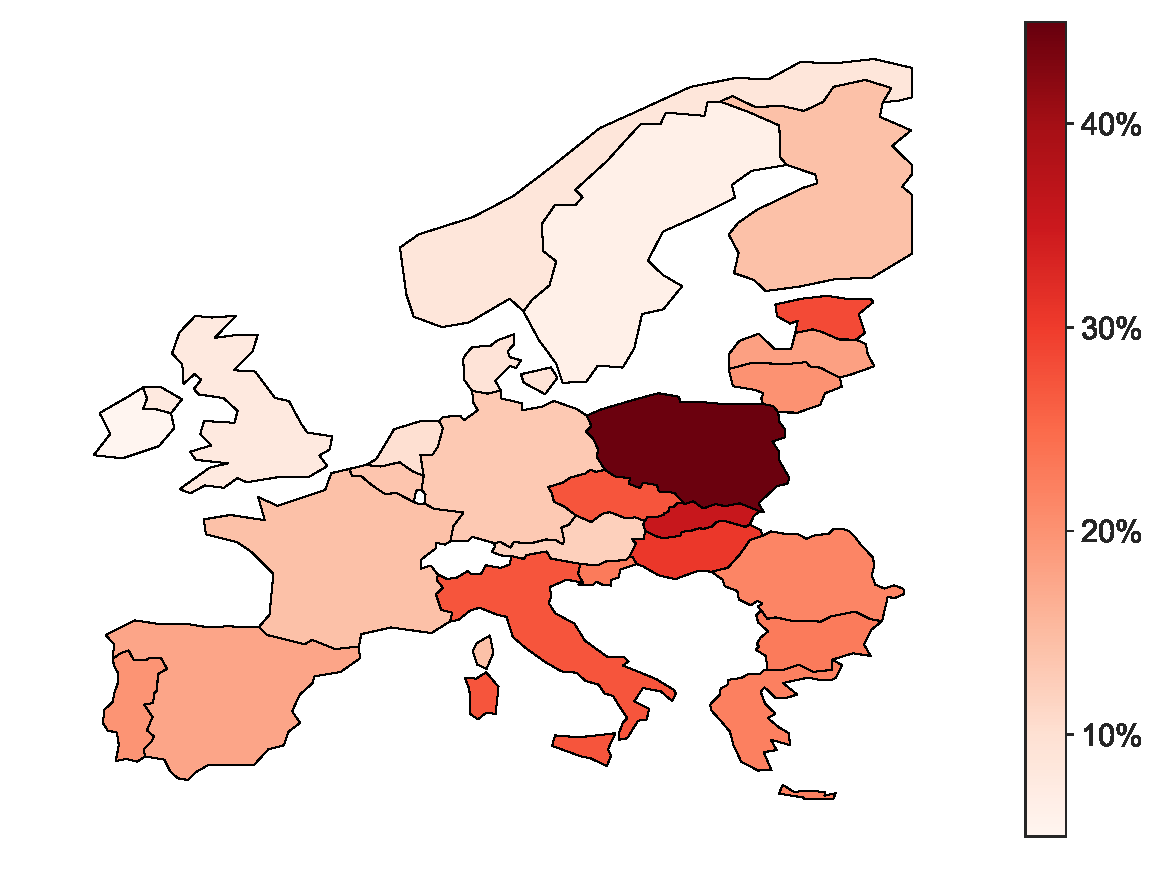
\includegraphics[width=.9\textwidth]{images/ted_networks/eu_sb_map.pdf}
\caption[Single bidding rates of EU countries.]{Single bidding rates of EU countries, 2008-2016.}
\label{fig:eu_sb_rates}
\end{figure*}


How does this measure correlate with the previously discussed survey-based measures of corruption risk? We find that national single bidding rates correlate significantly with a variety of corruption indicators discussed above, ranging in absolute value from .65 to .72.

\begin{figure*}[!ht]
\centering
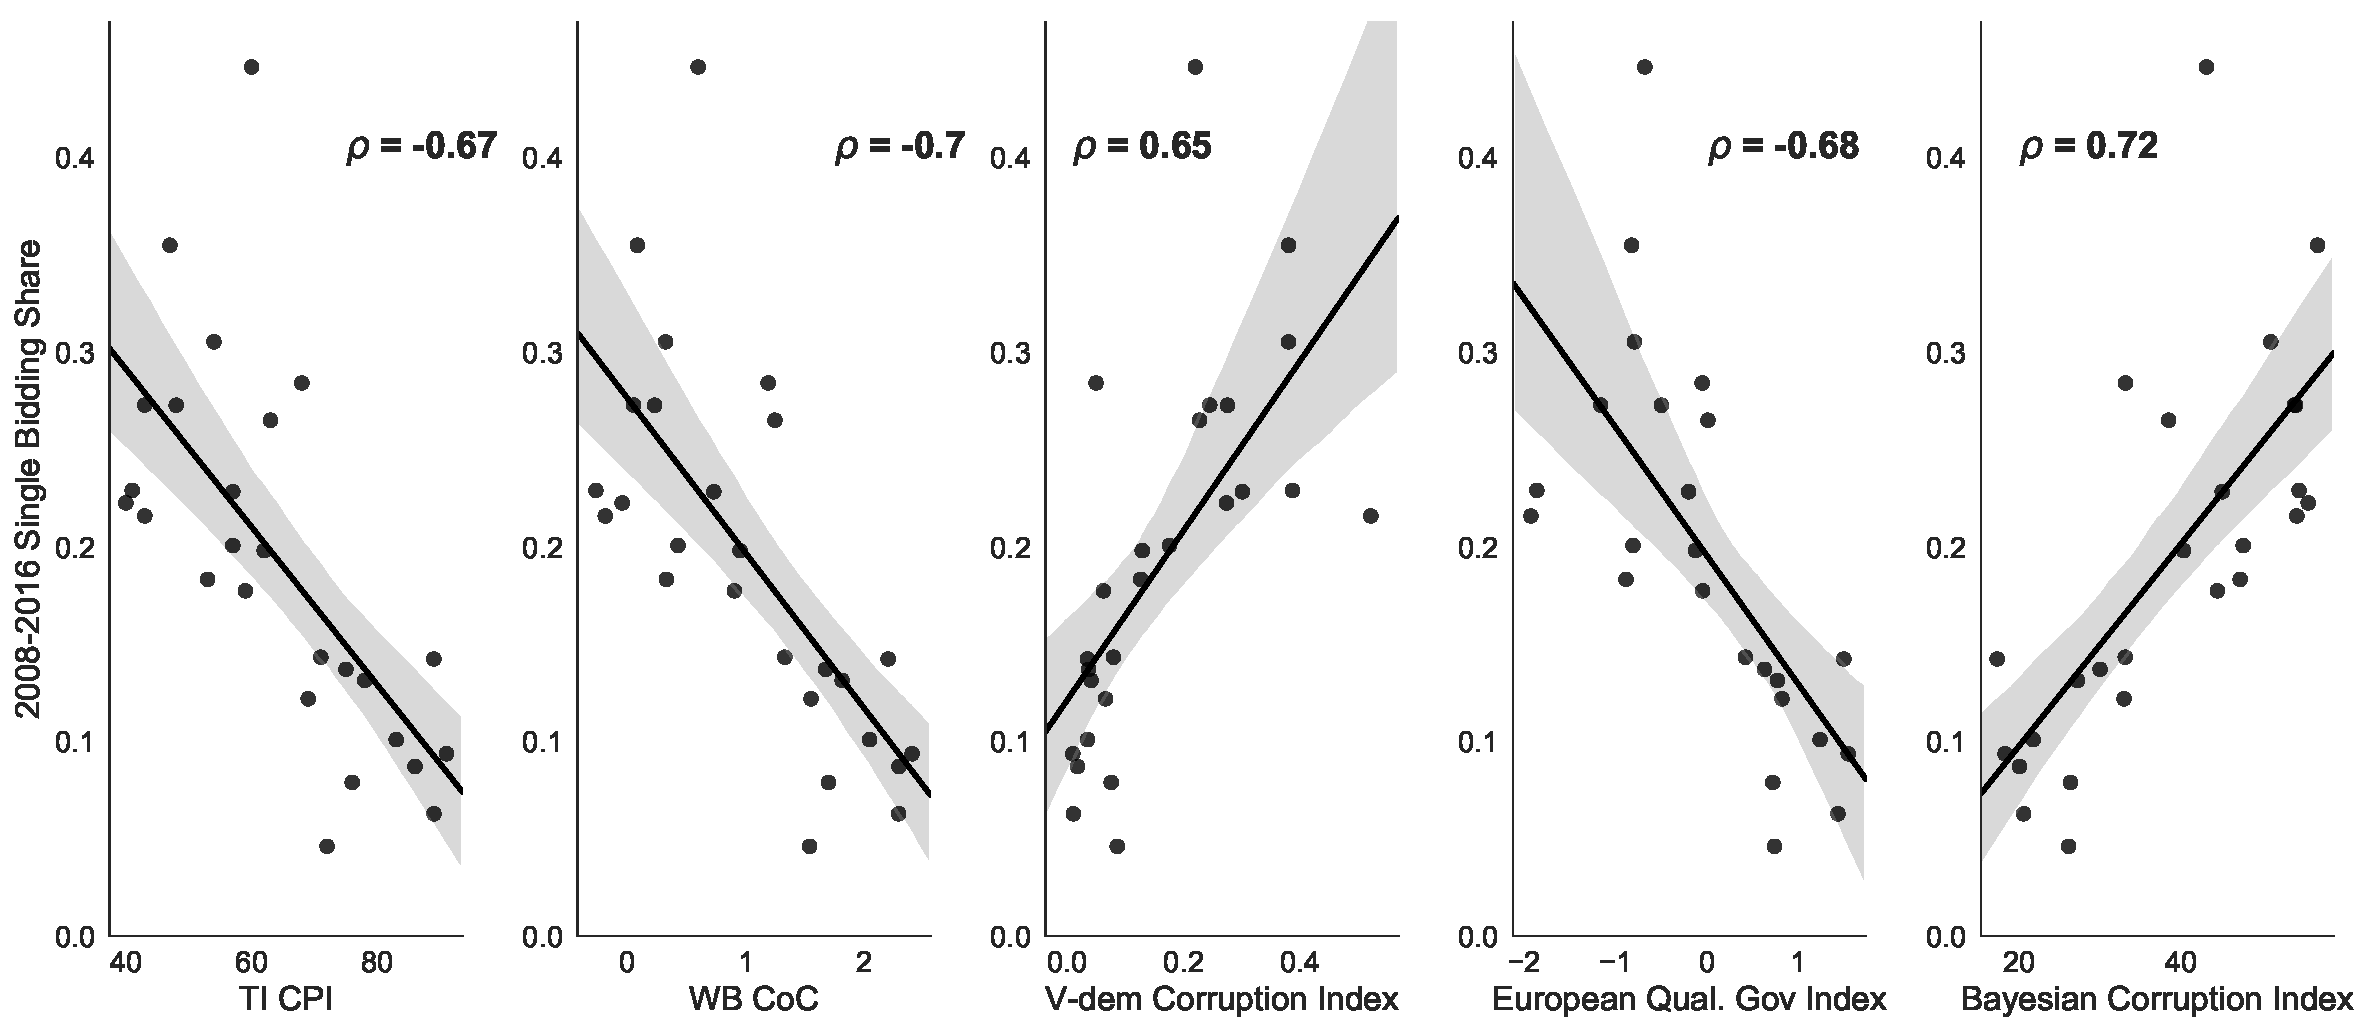
\includegraphics[width=\textwidth]{images/ted_networks/sb_corruption_correlations.pdf}
\caption[Correlates of national single bidding]{Correlation of national-level single bidding rates 2008-2016 with other commonly used measures of corruption in 2013. Where the correlation between the single bidding rate and the corruption indicator is negative the corruption indicator measures control of corruption and higher values indicate better outcomes.}
\label{fig:ted_sb_corr}
\end{figure*}


We will return to the national-level data in Chapter 4, in which we apply network science methods to describe the distribution of corruption risk in public procurement markets.

\section{Corruption as Networked Phenomenon}
We now turn our attention to past work on corruption, or criminal behavior more general, which employs network methods or perspective. Though we have mentioned network-based interpretations of the findings of related work in the previous sections, the works that we discuss now take an explicit network or relational approach to the study of corruption.

Many studies of organized crime, for instance the mafia represent the structure of the organization as a network~\cite{gambetta1996sicilian,calderoni2011strategic}, especially when transnational organizations are studied~\cite{williams2001transnational}. Network structure of contacts and command hierarchy reveal how these organizations function, how they structure themselves to be resilient to turncoats or attacks from rival organizations~\cite{agreste2016network,dellaposta2017network}. Similarly, networks provide a valuable perspective on the operation of terrorist cells~\cite{krebs2002mapping}.

White collar crime has also been studied using network methods. In an example from Canada, the diffuse network of actors responsible for various accounting procedures facilitated a significant corruption ring involving top members of a major political party~\cite{neu2013accounting}. Researchers have used email data from Enron, a major US Fortune 500 company which filed for bankruptcy in 2001 amid allegations of fraud and criminal conspiracy by its executives, to study patterns of communication during a crisis and criminal cover-up~\cite{diesner2005communication}.

In a more recent article, Ribeiro et al. investigated the temporal evolution of the network of co-conspirators in Brazilian political scandals over a 27 year period~\cite{ribeiro2018dynamical}. By the time of the Petrobras scandal, a giant connected component had emerged in the network of co-conspiracy, connecting a large majority of individuals. More broadly, network methods have been used to understand the co-occurrence of different sorts of criminality~\cite{tumminello2013phenomenology,rostami2015complexity}. For example, criminals often specialize in certain kinds of crimes (for instance financial crimes such as fraud) and tend to carry out new kinds of crime with accomplices who already have some experience. 
\pagestyle{fancy} %Literature review
% !TeX root = ../main.tex
\chapter{Extracting the multimodal fingerprint for transportation networks}

From bicycle paths to street and rail networks, mobility in cities increasingly relies on multimodality. These different modes of transportations can be conveniently described as multiplex networks, where layers are associated with different infrastructures. Here we show how to extract the multimodal blueprint of cities from their multiplex transportation networks. We identify clusters of cities with similar multimodal profiles, and link this feature to the level of sustainable mobility of each cluster. Our work highlights the importance of evaluating the transportation systems of a city altogether to correctly capture the nature of different urban clusters. 


\section{Prelude}
From a network perspective, the different modes of transportation can be described as a mathematical object, the multiplex transport network \cite{Morris2012,Strano2015,Aleta2017}. A city's multiplex transport network contains other network layers that have co-evolved with the street layer, such as the bicycle layer or the rail network layer, which together constitute the multimodal transportation backbone of a city. Due to the car-centric development of most cities \cite{Jacobs1961}, street layers are the most developed layers \cite{Gossling2016,Szell2018} and define or strongly limit other layers: For example, sidewalks are by definition footpaths along the side of a street and make up a substantial part of a city's pedestrian space \cite{Gossling2016}; similarly, most bicycle paths are part of a street or are built along the side. 

Here we consider the transport networks of 15 world cities and develop an urban fingerprinting technique based on multiplex network theory to characterize the various ways their transport layers are interconnected, outlining the potential for multimodal transport. Using clustering algorithms on the resulting urban fingerprints, we find clear classes of cities reflecting their transport priorities.

\section{METHODS AND DATA}
We acquired urban transportation networks from multiple cities around the world using OSMnx \cite{Boeing2017a}, a Python library to download and construct networks from OpenStreetMap (OSM). These data sets are of high quality \cite{Haklay2010b,Girres2010} in terms of correspondence with municipal open data \cite{Ferster2019} and completeness: More than $80\%$ of the world is covered by OSM \cite{Barbosa-Filho2017}.  The various analyzed urban areas and their properties are reported in Table~\ref{tab:Table1}. Figure \ref{fig:fig01} shows the different network layers for two of our analyzed cities. The pedestrian layer contains all sidewalks and pedestrian paths. The bicycle layer consists of all infrastructure exclusive to bicycles, like designated cycleways and bicycle trails. The rail network captures all public transportation that uses rails, including subways and tramways. Finally, the street layer is composed of all streets designated for motor vehicles.

\begin{table*}[ht!]
	\centering
	\begin{adjustbox}{width=0.6\textwidth,keepaspectratio}
		\begin{tabular}{lrrrrrrrrl}
			\toprule
			{} & \multicolumn{2}{l}{walk} & \multicolumn{2}{l}{bike} & \multicolumn{2}{l}{rail} & \multicolumn{2}{l}{drive} &  Population \\
			{} &     $N$ & $CC$ &    $N$ &  $CC$ &   $N$ & $CC$ &     $N$ & \multicolumn{2}{l}{$CC$} \\
			\midrule
			Amsterdam  &   23321 &    1 &  34529 &   355 &  1096 &    8 &   15125 &    1 &     872,680 \\
			Barcelona  &   20203 &    1 &   7553 &   122 &   249 &   15 &   10393 &    1 &   1,600,000 \\
			Bogota     &   81814 &    1 &   9760 &   171 &   166 &   12 &   62017 &    1 &   7,412,566 \\
			Budapest   &   73172 &    1 &  10494 &   257 &  1588 &   20 &   37012 &    1 &   1,752,286 \\
			Copenhagen &   30746 &    1 &  13980 &   321 &   276 &    3 &   15822 &    1 &   2,557,737 \\
			Detroit    &   47828 &    1 &   3663 &    53 &    20 &    3 &   28462 &    1 &     672,662 \\
			Jakarta    &  140042 &    1 &    248 &    19 &    58 &    6 &  138388 &    1 &  10,075,310 \\
			LA         &   89543 &    1 &  14577 &   230 &   173 &    9 &   71091 &    1 &   3,792,621 \\
			London     &  270659 &    1 &  62398 &  3023 &  2988 &   38 &  179782 &    1 &   8,908,081 \\
			Manhattan  &   13326 &    1 &   3871 &   105 &   349 &    5 &    5671 &    1 &   1,628,701 \\
			Mexico     &  108033 &    1 &   5218 &    52 &   370 &   17 &   95375 &    1 &   8,918,653 \\
			Phoenix    &  111363 &    1 &  35631 &   141 &   105 &    4 &   73688 &    1 &   1,445,632 \\
			Portland   &   50878 &    1 &  24252 &   198 &   230 &    2 &   35025 &    1 &     583,776 \\
			Singapore  &   82808 &    1 &  12981 &   104 &   683 &   14 &   50403 &    1 &   5,638,700 \\
			\bottomrule
			\end{tabular}
	\end{adjustbox}
	\caption{Measures for the administrative area of analyzed cities. The number of connected components ($CC$) and nodes ($N$) for each layer in all cities of our dataset are highly diverse due to the varying developmental levels and focus of transport. 
		\label{tab:Table1}}
\end{table*}

The codes to replicate the results are available as Jupyter Notebooks in: (\url{https://github.com/nateraluis/bicycle-network-growth}), and the data can be downloaded from Harvard Dataverse (\url{https://doi.org/10.7910/DVN/GSOPCK})

We characterize each city as a multiplex network \cite{Boccaletti2014,Kivela2014,Battiston2017a} with $M$ layers and $N$ nodes that can be active in one or more layers in the system. Layers are represented by a primal approach \cite{Porta2006} in which nodes are intersections (that may be present in one or more layers), while links represent streets (s), bicycle paths and designated bicycle infrastructure (b), subways, trams and rail infrastructure (r), or pedestrian infrastructure (p). This recent approach has been useful to demonstrate how cities grow \cite{Strano2012,Barthelemy2013}, how efficient \cite{Gallotti2014} and dense they are, and to capture the tendency of travel routes to gravitate towards city centers \cite{Lee2017}. Each layer $\alpha=1, \dots, M$ is described by an adjacency matrix $A^{[\alpha]}=\{a_{ij}^{[\alpha]}\}$ where $a_{ij}^{[\alpha]}=1$ if there is a link between nodes $i$ and $j$ in layer $\alpha$ and 0 otherwise. The multiplex urban system is then specified as a vector of adjacency matrices $\textbf{A} = (A^{[1]}, \ldots, A^{[M]})$.


\begin{figure*}[t!]
	\centering
	\includegraphics[width=\textwidth]{images/multiplex/Fig01.png}
	\caption{{\textbf (Map plots, left)} Networks representing various layers of transport infrastructure (pedestrian paths, bicycle paths, rail lines, and streets) for  Copenhagen and London, with data from OpenStreetMap. {\textbf (Right)} Connected component size distribution $P(N_{cc})$ as a function of the ranking of the component for all considered network layers and cities. All layers are well connected except the bicycle layer: Copenhagen has 321 bicycle network components despite being known as a bicycle-friendly city, while London's bicycle layer is much more fragmented, featuring over 3000 disconnected components. Copenhagen's largest connected bicycle component (leftmost data point) spans 50\% of the network, but London's only less than 5\%.}
	\label{fig:fig01}
\end{figure*}

\section{FINDINGS}
In a multimodal city, we expect to find many transport hubs that connect different layers, such as train stations with bicycle and street access, i.e. nodes that are active in different multiplex configurations. Note that even in a multimodally ''optimal'' city there will be a high heterogeneity of node activities due to the different speeds and nature of transport modes, implying, for example, a much lower density of nodes necessary for a train network than for a bicycle network. Here we build a way to see and compare all combinations of node activities in the system, that help us learn how much focus a city puts on connecting different modes. We can define such a fingerprint using the multiplex network formalism. We call the plot that counts the combinations of node activities a city's \emph{overlap census} (Figure \ref{fig:fig02}). Similar to edge overlap \cite{Bianconi2013,Battiston2014a} and multiplex motifs \cite{Battiston2017} that provide a characterization of multiplexity at the local scale, the overlap census captures the percentage of nodes that are active in different multiplex configurations and provides an "urban fingerprint'' of multimodality \cite{Aleta2017}.

\begin{figure*}[t!]
	\centering
	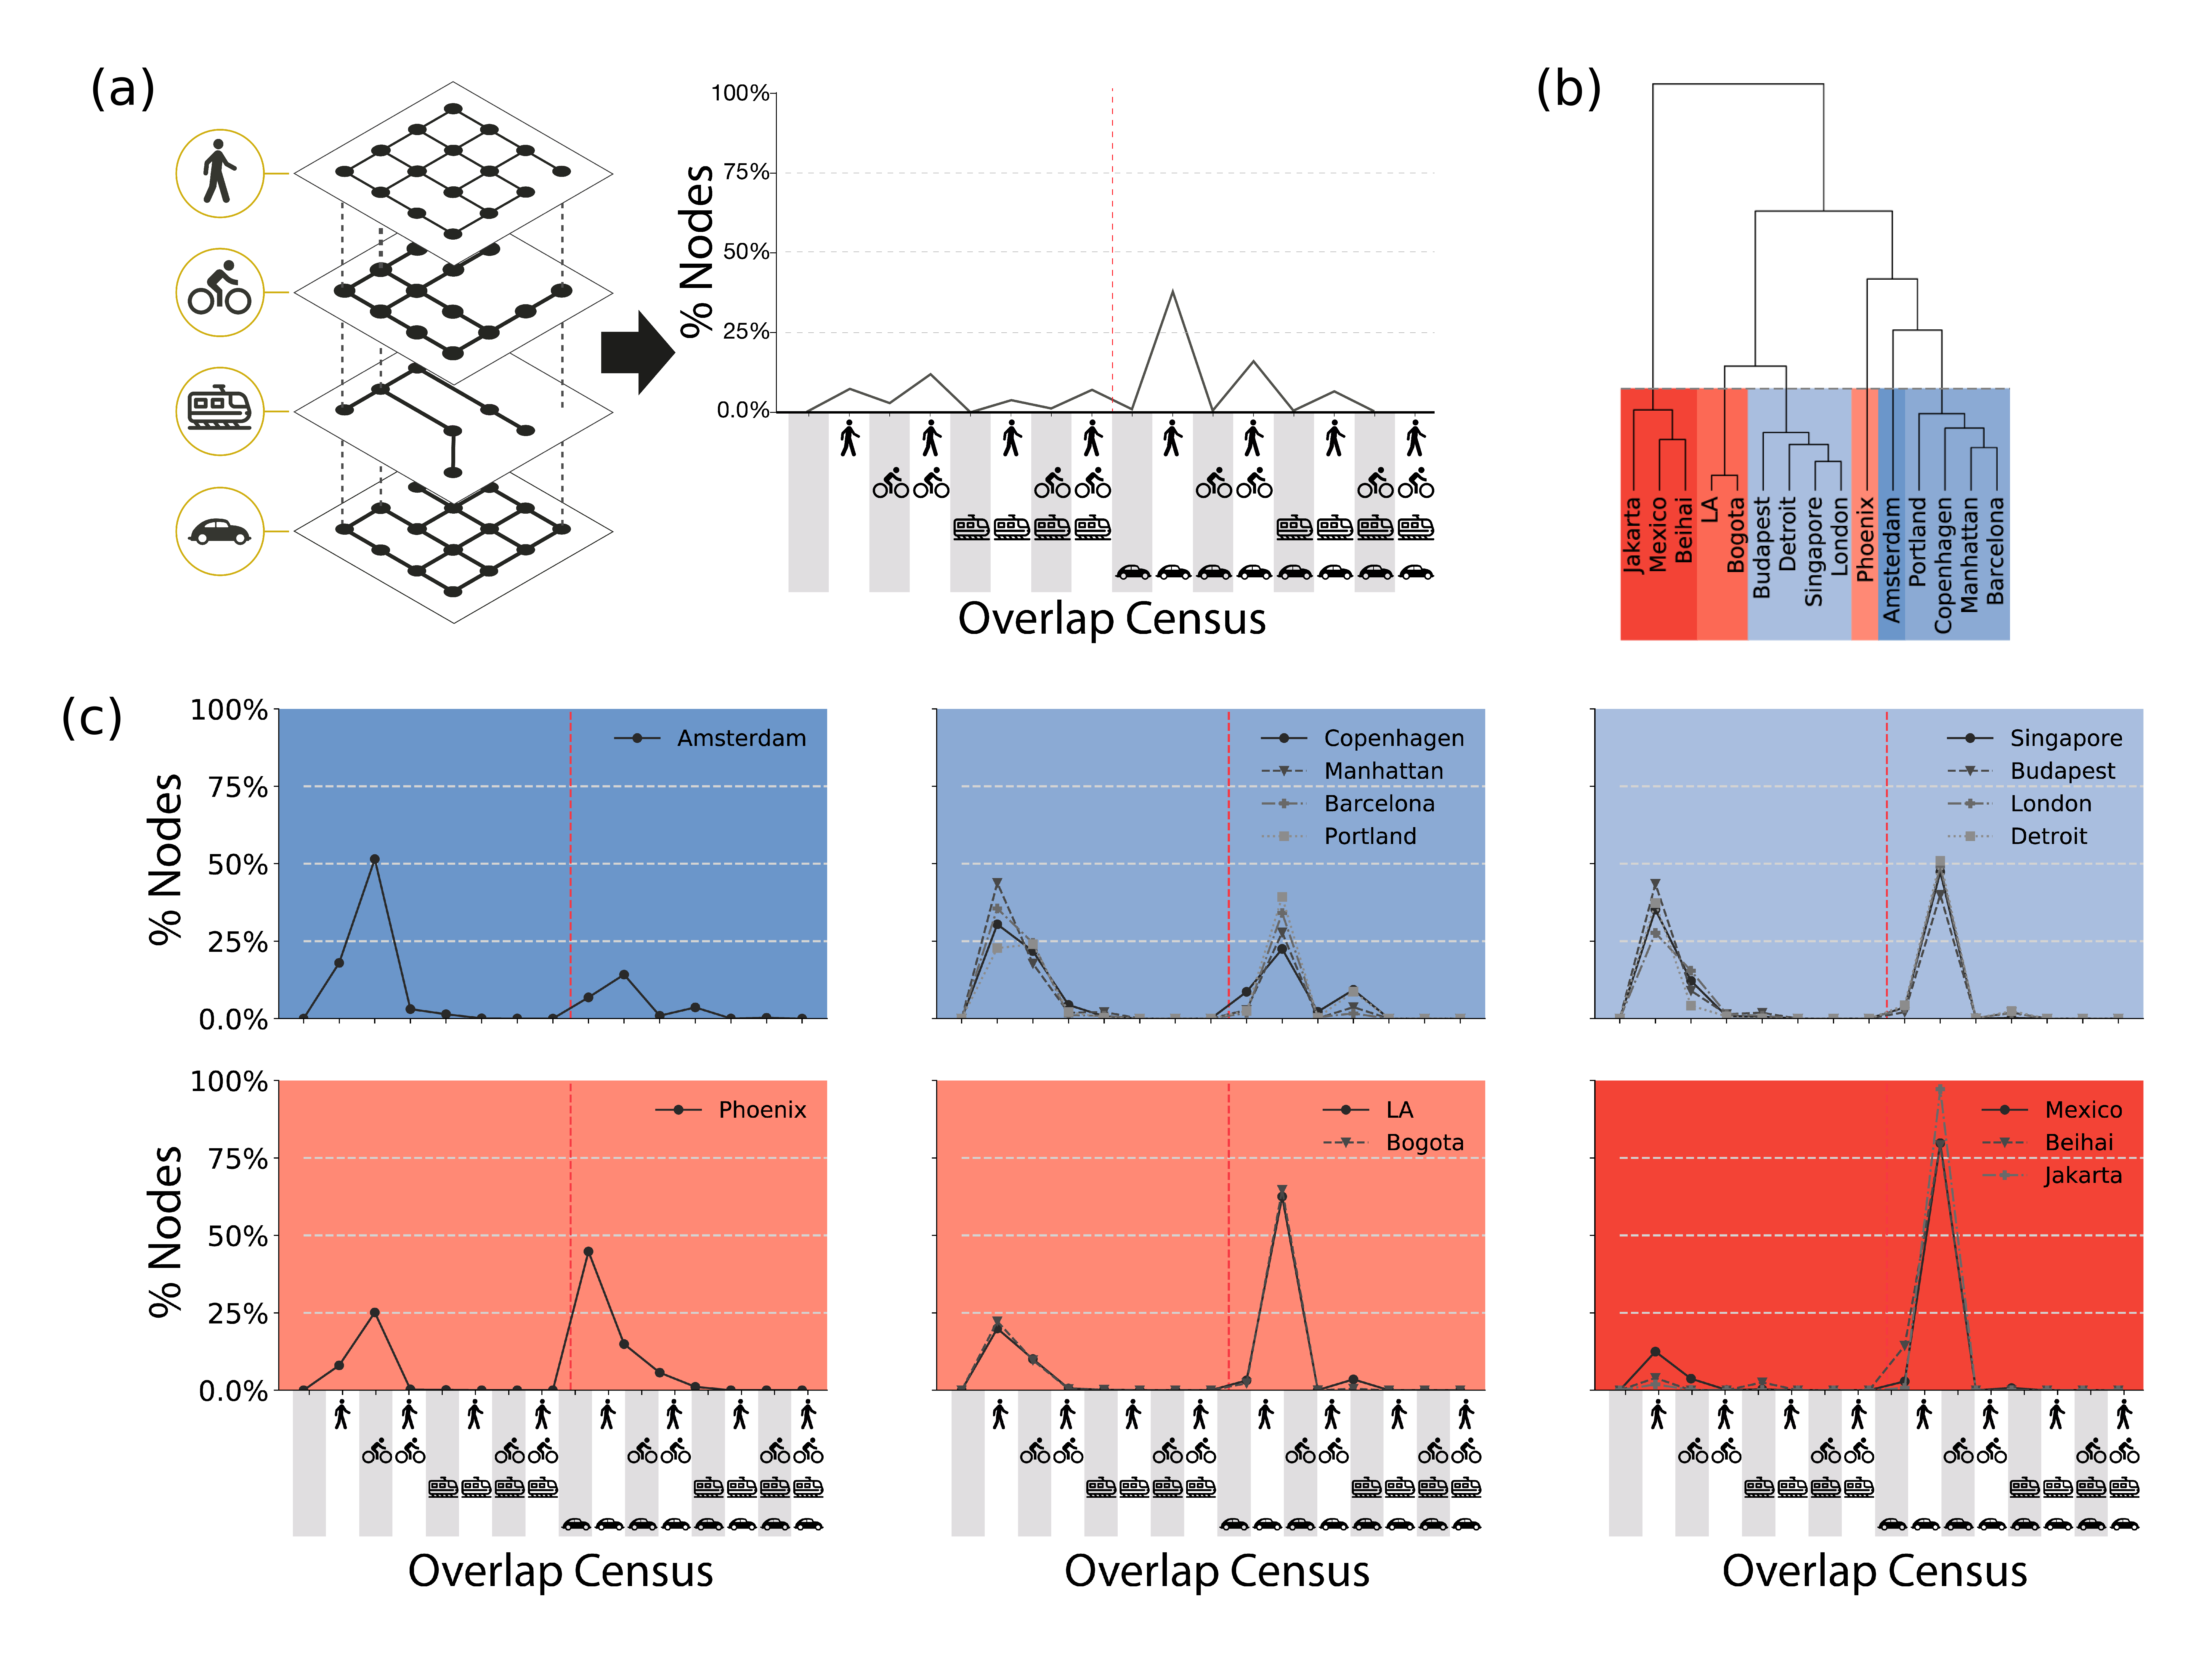
\includegraphics[width=0.8\textwidth]{images/multiplex/Fig02.png}
	\caption{
		\textbf{(a)} Schematic of multiplex layers in a city (left) and its transformation to the overlap census (right). In the overlap census, the vertical red line gives a visual separation of the left from the right half where nodes become active in the street layer. High spikes in the right half indicate car-centricity.
		 \textbf{(b)} Clusters of cities based on similarity of their overlap census. We find six different clusters using a k-means algorithm (coloured areas), which explain more than $90\%$ of the variance.
		 \textbf{(c)} Overlap census for cities in each cluster. The first one corresponds to Amsterdam (the city with most active nodes in bicycle-only configurations). The Copenhagen-Manhattan-Barcelona-Portland city cluster has many active nodes in pedestrian-only and bicycle-only configurations, representing an active mobility city. The clusters of Los Angeles-Bogota and Mexico-Beihai-Jakarta are car-centric.}
	\label{fig:fig02}
\end{figure*}

To define the overlap census formally, we calculate the degree of each node in layer $\alpha$ as $ k_i^{[\alpha]}=\sum_ja_{ij}^{[\alpha]} $. We store degrees in a vector for each layer, \textbf{\textit{k}}$^{[\alpha]}=(k_i^{[\alpha]}, \dots, k_n^{[\alpha]})$, indicating layers by `p' for pedestrian, `b' for bicycle, `r' for rail infrastructure, and `s' for streets, as before. The use of vectorial variables like \textbf{A} and \textbf{\textit{k}}$^{[\alpha]}$ instead of those of the aggregated network lets us capture the richness of the system and work in the various layers independently. Given a Multiplex transport network with $M$ layers the overlap census is a vector of $2^{M-1}$ components, which accounts for the fractions of nodes that can be reached through at least one layer.

In Fig.~\ref{fig:fig02}(a) we show a schematic of how the overlap census is built: taking the multiplex network, transforming it to its corresponding degree vectors for all layers in the system, and calculating the percentage of nodes that overlap in different configurations. Note that the overlap census provides more information than a simple counting of nodes, edges, or other single-layer network measures. The multiplex approach addresses the multimodality of a city: it not only counts how many nodes or links there are in each layer, but it shows how they are combined, revealing the possible multimodal mobility combinations in the city. Understanding the possibilities for interchange between mobility layers provides us with a better understanding of urban systems, showing us the complexity and interplay between layers.

A good way to assess a city's overlap census is by comparing it with the overlap census of other cities. Explicitly, we find similarities between cities via a k-means algorithm. The algorithm separates the 15 analyzed cities into six different clusters [Fig.~\ref{fig:fig02}(b)]. On the left half of the overlap census, we show the configurations in which nodes are not active in the street layer, while the right half contains car-related configurations. These clusters of cities are useful to explain similarities in infrastructure planning in different urban transport development paths \cite{Rodrigue2013,Louf2014}, with clusters of car-centric urbanization (like Mexico, Beihai, and Jakarta) opposed to clusters that show a more multimodally focused evolution of their urban mobility infrastructure (like Copenhagen, Manhattan, Barcelona, and Portland). In the extreme cluster that contains only Amsterdam, close to $50\%$ of nodes are active in the bicycle layer, while in the Mexico-Beihai-Jakarta cluster more than $50\%$ of nodes are active in the street-pedestrian configuration. This concentration of nodes in just one configuration informs us not only about the (sometimes already well-known) mobility character of the city, i.e. Amsterdam being a bicycle-friendly city, but unveils the importance of explicitly considering overlooked layers and their interconnections. For example, Singapore, Budapest, London, and Detroit have two main peaks indicating that most of their nodes are either active in the street-pedestrian or only in the pedestrian configuration, i.e. there are plenty of walkable areas exclusive to pedestrians. This is not the case in Los Angeles and Bogota, where the majority of nodes are active in the car-pedestrian combination, i.e. the pedestrians have to share most of the city with cars.\pagestyle{fancy} %Multiplex fingerprint
%% !TeX root = ../main.tex
\chapter{Life quality as walkability}

\section{Prelude}

During the 20th century, most cities have evolved to accommodate a car-centric vision \cite{Jacobs1961}, allocating a privileged amount of urban space to motorized traffic \cite{Gossling2016,Szell2018}. From a liveability perspective, this situation is suboptimal because the automobile infrastructure dominates and defines the walkable area, increasing car traffic, air pollution and deteriorating walkable conditions.

The concept of walkability is an important factor to consider in connection with liveability. Liveability refers to an environment from an individual perspective \cite{Heylen2006} which includes "a vibrant, attractive and secure environment for people to live, work and play and encompasses good governance, a competitive economy, high quality of living and environment sustainability” \cite{Shamsuddin2012}. Thus in a liveable city, there must be an emphasis not only on sustainable transportation and built environment to reduce the harm on nature \cite{Campbell1996,Jabareen2013} but also encouraging citizens to walk for supporting their physical and mental well-being \cite{Frank2006}. However, improving walkability is more complex than we would think. Walking should be an available, safe and well-connected mode of transportation, but as Speck put it well, it should be interesting and comfortable as well, to have a feeling of the streets as ’outdoor living rooms’ \cite{Speck2012}.

The pedestrian infrastructure that sustains walkability in a city can be described as a network \cite{Porta2006}. This approach has been useful to identify street patterns \cite{Barthelemy2008,Louf2014b} and its evolution \cite{Strano2012,Barthelemy2013}, measure the morphology of cities \cite{Boeing2018}, and how the streets connectivity impacts on pedestrian volume \cite{Hajrasouliha2015}.

The various approaches to create a walkability index or so-called walk score consider mainly the following components: safety and security \cite{Quercia2015,Silva2018}; convenience, attractiveness and public policy \cite{Krambeck2006,Speck2012}, connectedness \cite{Southworth2005}, but also reckon with the land use mix and residential density of the certain area\cite{Carr2010}. Another approximation rather accents the importance of its effect on air pollution, health problems, travel costs and even on the sense of community\cite{Stephen2004}. Thus measuring walkability not only captures the propensity to walk in a city but also includes the components a liveable city must have and support, under the umbrella of sustainability.

There are good examples of how sustainable city development initiatives tackle growing inequalities with data-driven approaches. Long Island used city data to analyze which amenities are needed to increase the quality of life in a newly built environment \cite{LongIsland}, other cities are investing in smart technologies to develop public transport, connecting spatially discriminated areas \cite{NYC,Amsterdam}.

Since the number of components which should be taken into consideration in creating a walkability index is high, the types of data are also mixed and thus difficult to integrate. While the information on connectedness, security, residential density, etc. is quantitative and in general easily available, gaining opinion about attractiveness, convenience, or even about the feeling of security is more complicated. Here we propose to use a data-driven approach as a proxy to quantify life quality, making it reproducible and easily expanded to include different data sources. We apply our methods to Budapest, but as having an emphasis on the online and easily available quantitative data, the methods can be generalized and applied to any city.

\section{Data}
We work with three different data sources: networks, points of interest and city attributes. The pedestrian network and points of interest were acquired using OSMnx \cite{Boeing2017a}, a python library to download and construct networks from OpenStreetMap (OSM). The data contained in OSM is of high quality \cite{Haklay2010b,Girres2010} in terms of correspondence with municipal open data \cite{Ferster2019} and completeness: More than $80\%$ of the world is covered by OSM \cite{Barbosa-Filho2017}.

The majority of points of interest were downloaded from OpenStreetMap, from different classification keys (amenity, tourism, shop, office, leisure) using OSMnx \cite{Boeing2017a}. We filtered the points of interest using the districts' demarcation \cite{hu_dist}, to get only the data within Budapest boundaries, having, as a result, more than $39,000$ data points. We complement the data sets with secondary data sources as specialized directories of doctors and childcare facilities (see appendix).

We categorize the points of interest in six main categories: I) Family friendliness (Access to education and daycare, and family support services), II) Access to health care and sport facilities, III) Art and culture (e.g.: museums, exhibitions), IV) Nightlife (e.g.: bars, restaurants), V) Environment (air quality and access to green areas), and VI) Public Safety. The points of interest and secondary data sources are available at \url{https://github.com/nateraluis/Budapest_LQI}

The district-level data (population and crimes) were obtained from the Hungarian Police's public database, calculated based on the number of crimes committed in public places 100 thousand per capita in 2018 \cite{hun_police}. Population data is coming from the 2016 micro-census conducted by the Hungarian Statistical Bureau \cite{hun_pop}. We took into account the air pollution, this data set coming from National Air Pollution Measurement Network \cite{hun_env}, containing the geolocation of the air quality stations and different measures (annual median concentration of carbon monoxide, nitrogen dioxide, and PM10 dust).

Accuracy of the Life Quality Index (LQI) model highly depends on how comprehensive the distribution of listed services. We use OSM as our key data source, but to achieve a more comprehensive and country-specific database we collect publicly available data from various Hungarian websites for each category (See Appendix A for databases and sources)

The network contains all the sidewalks and pedestrian designated infrastructure, it is conceptualized as undirected, nonplanar and primal network \cite{Porta2006}. The pedestrian network is described as a weighted graph, with its adjacency matrix $W=w_{ij}$ where the weight $w_{ij}$ contains the length between $i$ and $j$ if connected, and $0$ otherwise.

We assigned properties to the nodes of the network, matching the nodes with their corresponding districts, then assign nodes as attributes based on the district level data (population and crimes, see section \ref{safety}). For the pollution data, we calculated the corresponding Voronoi cells, for the air quality stations, and matched the nodes with them, we divided the pollution by the number of nodes in each corresponding cell and assigned the value to the nodes (See section \ref{environment}). For the edges, we encoded their length $\ell_{ij}$ along with the traversal time $Tt_{ij}$ between nodes $i$ and $j$ calculated as $Tt_{ij}=\frac{\ell_{ij}}{ps}$ where $ps$ is the pedestrian speed as a constant rate of $5km/h$.
\begin{figure*}[htbp]
	\centering
	\includegraphics[width=0.8\textwidth]{images/lqi/Budapest_Network_voronoi_op2.png}
	\caption{\textbf{(a)} Network representing Budapest pedestrian structure. The network was built following a primal approach, where the edges are sidewalks and pedestrian infrastructure, and nodes are intersections. \textbf{(b)} The graph-Voronoi tessellation of the Budapest network, generated using a subset of 15 parks as seeds. The color of the nodes represents the cell they belong to and the highlighted red dots are the seeds of each cell. The distance measure between two points is defined as the weighted shortest path on the graph, the weights being the average time required to cross a given edge.}
	\label{fig:BPnetwork}
\end{figure*}

\section{Quantifying Life Quality}
The life quality of a person is largely subjective and hard to quantify. However, it is both intuitive and has been scientifically shown that the environment and personal well-being strongly correlate \cite{rosow_1961}. Thus using environmental factors as proxies, life quality and livability becomes quantifiable \cite{kahneman_2006}.

The main environmental factors we consider in our model are: the availability of services and amenities, the quality of the infrastructure, environmental factors and safety. The goal of our model is to quantitatively characterize the immediate environment of residents in the space of factors that affect life quality.

The fundamental framework of our model and our calculations is the network representation of Budapest’s pedestrian infrastructure. The nodes of the network represent intersections, while links are sidewalks and pedestrian infrastructure. The output of our model is an index, that characterizes every node of the Budapest network, giving a high-resolution quality-landscape of the city. The index is ultimately a number aggregated from multiple sub-categories, and its main value is highlighting inequalities and relative deficiencies within the city.

The final value of the index is a weighted sum, characterizing every node (intersection) in the network:
\begin{equation} \label{final_Q}
    Q_i =w^{services}\Tilde{Q}_i^{services} + w^{safety} \Tilde{Q}_i^{safety} + w^{environment}\Tilde{Q}_i^{environment}
\end{equation}
In the equation $i$ represents an individual node in the network. The \say{tilde} above the $Q$ terms means that the values of the different category indices are normalized within the category. The weights $w$ assigned to every term are arbitrary and are highly context-dependent. We include the weights used for producing the results of this paper in Appendix B.  All terms of the equation are discussed in the following sections.

\subsection{The services index: $Q^{services}$}
The number quantifying each node in terms of how well it is connected with amenities and services is a weighted sum of sub-categories as well.
\begin{equation}\label{Q_services}
    Q_i^{services} =\sum_c w^c Q_i^c
\end{equation}

where, $c$ denotes categories (family, culture, health, sport, and nightlife), and $w^c$ the importance (weight, see Appendix B) of category $c$.
Some categories, like family, have further subcategories. Even though we have also had data and made a separate analysis on tourism, its effects on life quality of the residents are ambiguous, so we decided to omit it from the index.\\

What sets categories apart is that they incorporate different sets of amenities, with a few overlaps. The details of the categorization of amenities are included in the Appendix. \\

For every service/amenity class we have a given set of points of interest (POI) along with where the amenities of that class are available, with exact geo-location. We assign every POI of a given amenity class (e.g supermarket, pharmacy, school, etc.) to the nearest node on the infrastructure network. Each set of POIs organically generates a spatial partitioning of the city with one partition per POI. The partition of a POI is the set of all the nodes from which that particular POI can be reached faster than any other POI of the same class.

Mathematically these partitions are called graph-Voronoi cells \cite{erwing_2000,Deritei2014}, where every node of a cell is assigned to its closest seed (POI). Distance, in this case, is not euclidean or geometric distance, but the distance on the network, where we use the weighted shortest path between two nodes as the distance measure. The weight of links is a temporal parameter encoding the average time required to cross the represented street from one end to the other, thus the weight is a simple product of average speed and length of the street. This is in principle very similar to the way navigation systems find routes between points. For an example of a graph-Voronoi partitioning see Figure 1 (b).\\
To assess how well connected a node is to amenities we consider the following factors:
\begin{itemize}
    \item How important is an amenity - weight ($w_a$)
    \item How long does it take to reach the amenity - time to reach ($t_ia$)
    \item Relatively how many nodes (or people) does the amenity share with - exclusivity ($P_a$)
\end{itemize}

From the three factors, the latter two are calculated using the city infrastructure network. The index for an amenity class, from the perspective of node $i$, is proportional with its importance (weight) and it is inversely proportional with the time to reach the closest POI from $i$ and with the degree of exclusivity.
\begin{equation}\label{q_i}
    q_i^a=\frac{w_{a}}{(P_a+1)(t_{ia}+1)}
\end{equation}

There can be certain singular cases when a Voronoi cell is empty ($P_a=0$, i.e. no residents in the area) or the node i in question is right at the POI ($t_{ia}=0$). To avoid anomalies in the index we added 1 to both parameters.

The index of one category is proportional to the sum of its amenity-indices (calculated in (\ref{q_i})). To treat this number on the right scale (in practice we can get very large and very small numbers) we take the natural logarithm of the sum across amenities.
\begin{equation}
    Q_i^c=log(\sum_a q_i^a):
\end{equation}

As we have mentioned earlier the final services index is the weighted sum of the indices of the sub-categories.
$$Q_i^{services} =\sum_c w^cQ_i^c $$
Finally we normalize the values of $Q^{services}$ so its values are comparable to the other values of the final $Q$ equation (\ref{final_Q}):
\begin{equation}
    \Tilde{Q}_i^{services} =\frac{Q_i^{services}+|min(Q^{services})|}{max(Q^{services})+|min(Q^{services})|}
\end{equation}

\subsection{Safety index: $Q^{safety}$} \label{safety}

The safety index is calculated across districts based on the number of crimes committed per one hundred thousand residents. Since the highest resolution data available to us was on the district level, every node $i$ in the same district will have the same safety index value. The crime index:

$$Q_i^{crime}=\frac{N^{district}_{crime}}{n_i^{district}}$$
Where $N^{district}_{crime}$ is the number of crimes committed in a district in a year, and $n_i^{district}$ is the number of nodes in the district. The safety index is one minus the normalized crime index.
\begin{equation}
    \Tilde{Q}_i^{safety}=1-\frac{Q_i^{crime}}{max(Q^{crime})}
\end{equation}

\subsection{Environmental index $Q^{environment}$} \label{environment}
The environmental index is made up of two components: air pollution ratio and ratio of natural areas.

\subsubsection{Air pollution ratio}
We use the data provided by Budapest’s air pollution measuring stations for the year 2018. For this study, we used the yearly median value of three polluters: carbon monoxide, nitrogen dioxide, and PM10 dust-pollution.
As an approximation, we project the geometric Voronoi cells of the measuring stations onto the city map and each node will receive the pollution metrics of the geometrically closest station. We divide these values with the yearly upper health limit for the given polluter to assess to what degree do these values approximate the health limit. Thus the air pollution index of one node is formalized as follows:
$$C_i=\frac{c_i^{CO}}{c_{limit}^{CO}}+\frac{c_i^{NO_2}}{c_{limit}^{NO_2}}+\frac{c_i^{Pm10}}{c_{limit}^{Pm10}}$$

Where $c^{CO}_{limit}=3000 g/m^3$, $c^{NO_2}_{limit}=40 g/m^3$ , $c^{Pm10}_{limit}=40 g/m3$ are the yearly upper limits based on \cite{levegominoseg}.

\subsubsection{Ratio of natural areas}
For this index, we have data on the neighborhood level, which is a more granular level of administrative partitioning the city than the districts are. In this case, we project the same index onto every node in the same neighborhood. We consider as natural areas forests, parks and water surfaces (ponds, rivers, etc). \\
The index:
$$T_i=\frac{R_{water}^{nh(i)}+ R_{forest}^{nh(i)}+R_{park}^{nh(i)}}{max(T)}$$
Where $R_x^{nh(i)}$ is the relative surface area of natural area $x$ within the neighborhood that $i$ belongs to ($nh(i)$). In other words, the surface area of a natural area is divided by the number of nodes in the neighborhood and the surface area of the neighborhood. Thus
$R_x^{nh(i)}=\frac{T(x)}{T(nh(i))n_{nh}}$, where $T(x)$ is the surface area of $x$ natural area, $T(nh)$ is the surface area of $nh$ neighborhood and $n_{nh}$ is the number of nodes in neighborhood $nh$.
The final environmental index:
$$Q_i^{environment}=\frac{1+T_i}{1+C_i}$$,
That after a normalization is:
$$\Tilde{Q}_i^{environment}=\frac{Q_i^{environment}}{max(Q^{environment})}$$


\section{Results}
We quantify life quality in terms of each category (family support, education healthcare, sport, culture, nightlife, environment), and an overall measurement which contains all 6 categories and crime rate normalized by the population for the city of Budapest. Our method allows us to measure life quality for each intersection of the city, which helps to capture within neighborhood inequalities too. Analysis on the category level is beneficial for targeted policy interventions for better service allocation.

\begin{figure*}[htbp]
	\centering
	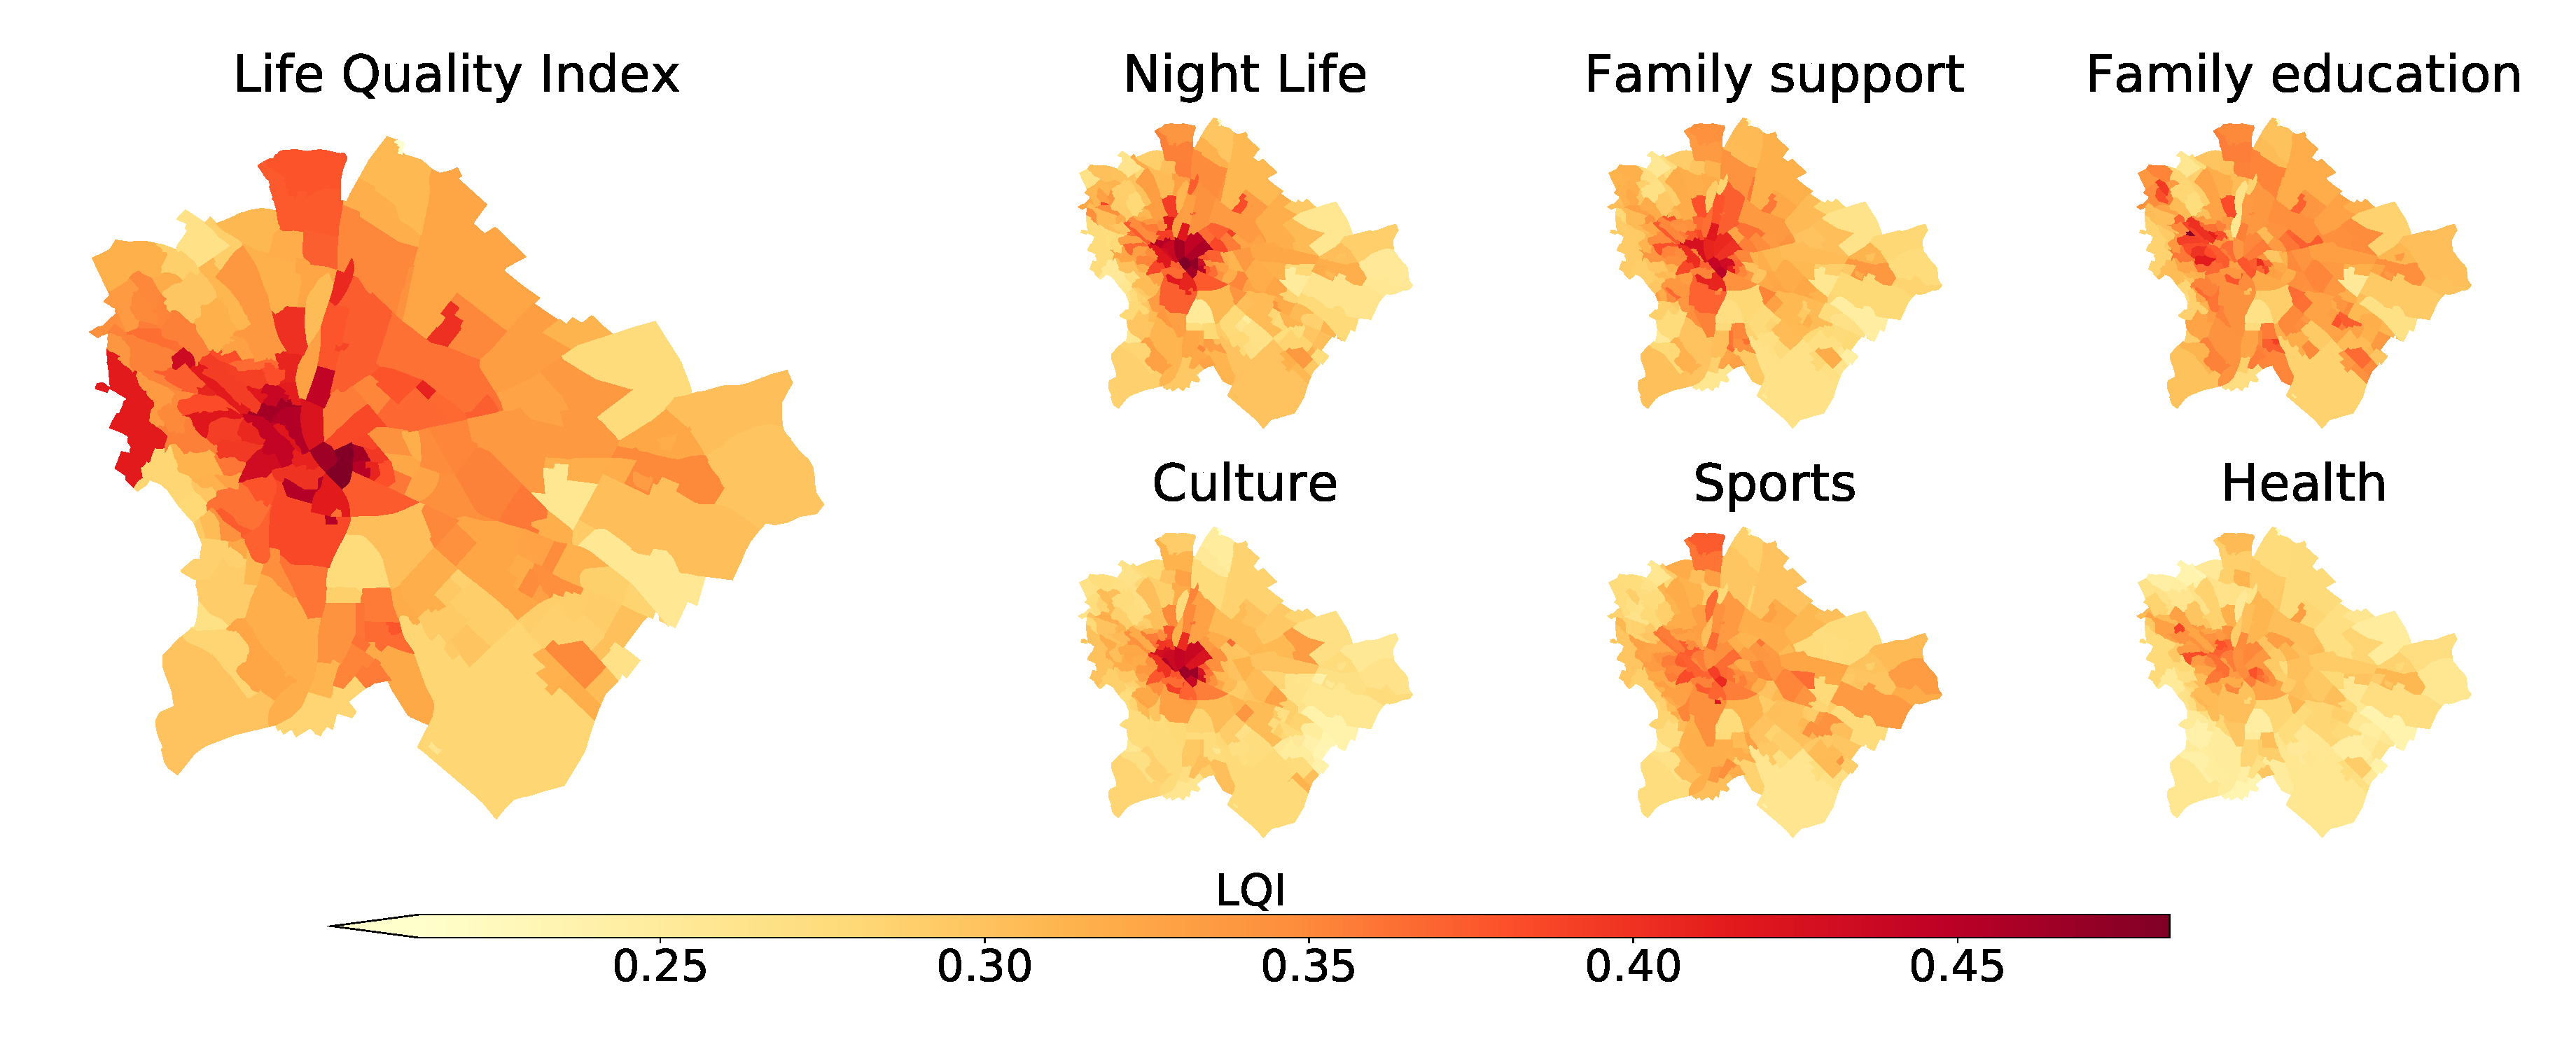
\includegraphics[width=0.8\textwidth]{images/lqi/Budapest_LQI_Neighborhoods-eps-converted-to.pdf}
	\caption{Budapest neighborhoods, average life quality by categories and aggregated life quality index.}
	\label{fig:BPlqi}
\end{figure*}

Figure~\ref{fig:BPlqi} shows our overall life quality index (LQI) and by categories. Heatmaps reveal important features of Budapest. Similarly to most European cities life quality is much better in the inner districts \cite{Hohenberg1986,Brueckner1999}, especially in the case of Night Life and Culture.

Budapest is divided by the Danube river into two main parts: Buda and Pest. The river does not only serve as a geographical border but due to historical reasons, it also divides the citizens by social status. Hilly Buda, on the West side of the river, used to be the capital of the country, with the residence of the former Hungarian king. On the other side, the mainly flat Pest used to be the agricultural supporter of the aristocrats in Buda \cite{Gyani}. Even though the city has changed dramatically since the Monarchy, the division of Buda and Pest persists, and our life quality index captures it well. However certain services are legally guaranteed to be evenly distributed in the city, such as education and healthcare, for precise modeling one should take into account private care too, which highlights inequalities. So, the traditional division of Buda and Pest is even visible in categories where there should not be that much of a difference (Education, Family Support, Healthcare).

Results also highlight that category LQI-s are highly correlated, less liveable neighborhoods are constant regardless of the amenity category, and well-performing neighborhoods do not change either. It is caused by two main factors: the lack of amenities and the relatively high walking distances in the suburbs.

The compact city concept focuses on building more sustainable and livable cities while designing practical neighborhoods where citizens can maintain everyday life without a car \cite{Dittmar2012}. Since, the walkability of a neighborhood highly correlates with its liveability \cite{Rogers2011} and the suburbs in Budapest do not show any compact city design features, both long distances and the lack of amenities effects suburban habitats lives negatively.

\subsection{Evaluation}

Multiple methods have been developed to evaluate the accuracy of quality of life metrics: Scholars used expert validation with geographic visualization \cite{Rinner2007,Gavrilidis}, correlations with socioeconomic characteristics \cite{Talen} and surveying citizens’ perceptions of the conditions of life \cite{Santos}.

Our evaluation is based on the micro-economical {\it hedonic approach} of estimating the values of public goods. In a capitalist market, real estate prices reflect the recognition of a neighborhood's characteristics: Prices are formed based on demand, more desirable places are more expensive, due to the underlying assumption of providing a higher quality of life. \cite{Brueckner1999} Estimating neighborhoods life-quality with real estate prices has a long tradition in urban literature \cite{Roback,Hoehn,Lora}, therefore we adopt this method to evaluate our model.

We collected the average $m^{2}/EUR$ price for all 23 districts of Budapest in January 2019 \cite{real_price} and correlated each LQI category averaged by district with it. Figure \ref{fig:LQI_ev} shows that our overall LQI correlates the most (R=0.91) with the real-estate prices. Most of its components have a positive correlation with real-estate prices, except the environment which is calculated based on air pollution and green surface proximity. The life quality (LQI) in Budapest is much higher in densely populated downtown districts, which are lack of green surface and suffers from high air pollution due to heavy traffic.

\begin{figure*}[htbp]
	\centering
	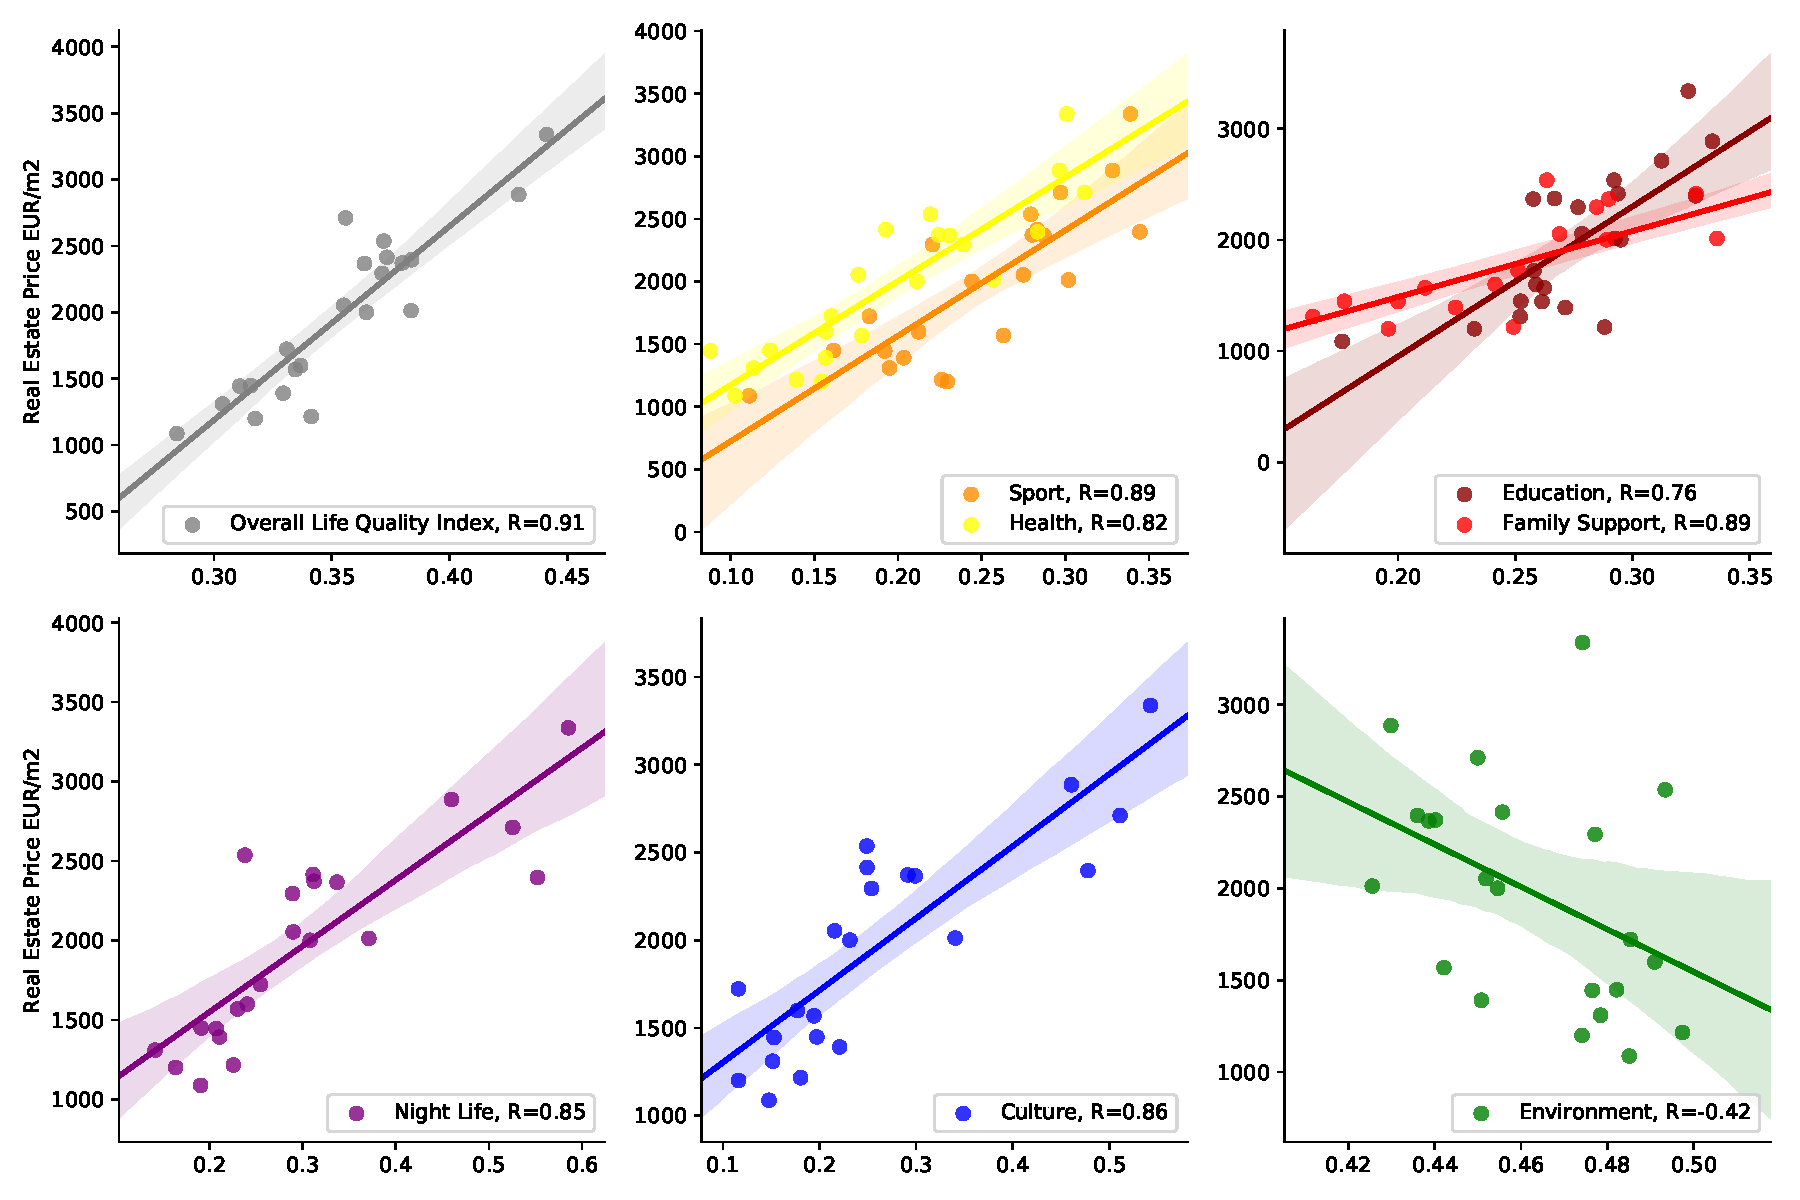
\includegraphics[width=0.8\textwidth]{images/lqi/LQI_categories_regplots.pdf}
	\caption{Districts of Budapest Life Quality Index (LQI) and its components correlated with real estate prices ($m^{2}/EUR$)}
	\label{fig:LQI_ev}
\end{figure*}

\paragraph{Summary} Locals of Budapest, like in most European cities, traditionally values downtown areas. The relative closeness to CBD, good access to public transport, and vital city life kept it as a desirable area for living \cite{Cassiers2012}. However, in recent years, the city is facing new challenges: due to gentrification \cite{Garcia} and over-tourism (eg.:Airbnb) real estate prices are sky-rocketing in downtown areas. In contrast with the early 2000-s when (upper) middle-class moved to the suburbs, nowadays, lower-income families and young professionals are leaving the downtown behind in hope for more affordable living.

As our findings show, Budapest is quite centralized and the quality of life highly correlates with real estate prices, which possibly lead to even more inequalities in the future. This spatial discrimination with longer traveling time, less fulfilling environment, and potential segregation reduces the chances of upward mobility and the quality of life of individuals \cite{Gobillon}.

\section{Discussion}
We have proposed a methodology to quantify life quality as a function of walkability on urban networks. We have used open data to capture inequalities between neighborhoods and districts in the city. We have shown that the real estate market reflects the life quality that our methods found.

A data-driven approach for quantifying life quality at such a granular level like our proposed method can help decision-makers to tackle social and environmental challenges better. Designing compact, liveable neighborhoods, considering also the upcoming environmental crisis is the number one priority of many cities worldwide.

The use of open data sources and algorithmic approaches adds up towards a systematic framework for understanding urban liveability. Our current approach is not the last word in this development since it does not yet account for multiple other variables, such as the quality of services and infrastructure, and other qualitative variables. To capture the more specific indicator of liveability in different cities it would be necessary to work with more granular and city-dependant data.

We anticipate a future stream of research focused on the use of worldwide open data sets to quantify urban liveability, including longitudinal studies in multiple cities, along with algorithmic modeling, simulations, and machine learning approaches, to first quantify the liveability, propose changes and test them with the ground truth data.
\pagestyle{fancy} %LQI walkability
%\chapter{Cartels}


Competing firms can increase profits by setting prices collectively, imposing significant costs on consumers. Such groups of firms are known as cartels and because this behavior is illegal, their operations are secretive and difficult to detect. Cartels do face a significant internal obstacle: members face short-run incentives to cheat. Here we present a network-based framework to detect potential cartels in bidding markets based on the idea that the likelihood that a group of firms can overcome this obstacle and sustain cooperation depends on the patterns of its interactions. 

We create a network of firms based on their co-bidding behavior, detect interacting groups, and measure their cohesion and exclusivity, two group-level features of their collective behavior. Applied to a market for school milk, our method detects a known cartel and calculates that it has high cohesion and exclusivity. In a comprehensive set of nearly 150,000 public contracts awarded by the Republic of Georgia from 2011 to 2016, detected groups in the high cohesion and exclusivity region are significantly more likely to display traditional markers of cartel behavior. We replicate this relationship between group topology and the emergence of cooperation in a simulation model. Our method presents a scalable, unsupervised method to find groups of firms in bidding markets ideally positioned to form lasting cartels.\footnote{This chapter partially draws on work that is under review at a journal at the time of submission of the thesis. No preprint is yet available.}.

This investigation contrasts with the previous chapters on corruption in that collusion is not a crime bridging the public and private sectors. In this sense the chapter and its findings represent a transfer of the network-based approach to the study of corruption to a related, parallel domain. 

We do note several important similarities between ``classic'' corruption in procurement and collusion. The first is that both require coordination in secret. The second similarity is that both activities are illegal, so participants face similar dilemmas. Third, the two often coincide as cartel may develop insider connections with bureaucrats~\cite{luz2017leniency} - recall that the Petrobras scandal involved a cartel of firms on the private sector side. Finally, both activities impose costs on the public. Therefore, though collusion is not usually considered to be the same as corruption, a better understanding of the emergence and sustenance of illegal collusion can inform us about corruption as well\footnote{A stand-alone version of this chapter is under review at a journal at the time of submission of the thesis.}.

\section{Prelude}
Cartels have been studied by economists since Adam Smith, who wrote that ``people of the same trade seldom meet together, even for merriment and diversion, but the conversation ends in a conspiracy against the public, or in some contrivance to raise prices.''~\cite{smith2003wealth} Competition between firms decreases profits, and so they have incentive to collude by setting prices or production collectively~\cite{marshall2012economics}. Three significant forces make running such a cartel difficult. First, they are generally illegal and are aggressively policed by competition authorities, presenting a significant obstacle to coordination. The second challenge is that cartels face a classic collective action problem: individual cartel members have short-term incentive to deviate from the collusive agreement. In the language of game theory, defection is a dominant strategy in the one-shot game. Finally, effective collusion requires unanimity, meaning that a single defector can significantly diminish the profits of the other cooperating firms.

Even though cartels face these internal and external threats to their stability there are many examples of cartels in a variety of industries from financial products~\cite{abrantes2012lessons} to vitamins~\cite{harrington2011private} operating successfully for long periods of time. Past research estimates that on average cartels increase prices by 20-30\%~\cite{connor2006cartel} and that in a given year a functioning cartel has a roughly 10\% chance of being discovered~\cite{combe2008cartels}, indicating that cartels are costly and that deterrence can be improved. In this chapter we propose a novel approach to the issue of detecting cartels using network methods, built on the idea that the network of firm-firm interactions can reveal hot-spots in which cooperation is easier to sustain. Groups of firms in these distinguished positions interact repeatedly and exclusively amongst themselves, creating ideal conditions to overcome their internal collective action problem.

Economists have long studied the market conditions under which cartels thrive, namely how they enable a cartel to overcome the problems of ``coordination, cheating, and entry.''~\cite{levenstein2006determines} For example coordination is easier in a smaller group with homogeneous firm sizes~\cite{compte2002capacity}, while frequency of interaction facilitates punishment of defectors, and high costs to entry insulate the cartel from outsiders~\cite{motta2004competition}. Another perspective on collusion is to consider that firms are playing a repeated prisoner's dilemma (PD) game~\cite{kofman1996aprisoner}. When choosing to compete (equivalently defecting from the cartel in the language of the PD) firms charge low prices, while when they collude (equivalently cooperate), they charge high prices. Collective profit is maximized if everyone colludes, but when colluding firms are undersold by even a single competing firm they fare badly~\cite{rapoport1974prisoner}. When players play multiple rounds of the PD, Axelrod demonstrated that cooperation can emerge as a winning strategy through learning and imitation~\cite{axelrod1981evolution}, a finding which replicates in the context of firms setting prices in oligopoly~\cite{dixon2002axelrod}. In the PD and many other games in which collectively optimal actions are personally costly to players, altruistic cooperation emerges under a variety of conditions through mechanisms such as reciprocity and the altruistic punishment of defectors or cheaters~\cite{bowles2011cooperative}.

Just as certain market conditions are known to favor cartels, researchers have observed that when players of the PD are arranged in some space or network which restricts their potential interactions, the potential for the emergence stable cooperation crucially depends on the structure of the space~\cite{nowak1993spatial,santos2008social,perc2013evolutionary,battiston2017determinants}. For example, correlations in the spatial distribution of agents have been shown to facilitate cooperation~\cite{szamado2008effect}. To the best of our knowledge, this observation that local correlation of interactions have significant influence on the emergence of cooperation has not been applied to the problem of detecting cartels.

We propose to apply network science methods to identify groups of intensely interacting firms in a market and to screen them for collusive potential, based on their network topology and how it may facilitate collusion. We focus on the case of collusion in public contracting markets, in which public bodies buy goods and services from private firms. These markets are vulnerable to collusion because of the inelasticity and regularity of government's demand for certain goods~\cite{pesendorfer2000,huschelrath2014cartel}. They are also large, accounting for between 10-20\% of GDP in the OECD~\cite{oecdprocurement}. Contracts are commonly awarded via auction to the lowest bidder. In these markets cartels often engage in bid-rigging, coordinating their bids to mask their agreement to avoid competition~\cite{porter1993detection}. 

Specifically, we use data on firms bidding for contracts to map in public contracting markets as networks of competing firms. We argue that such a network represents an embedding of the firms into a space which describes the competitive landscape of their industry or location, including its geography, technology, and scale. Within such co-bidding networks, we detect groups of firms whose local network topology are naturally conducive to sustaining collusion. Previous work on cartels has considered co-bidding networks of firms~\cite{toth2014toolkit,reeves2017bid,morselli2018network}, though none have used the network topology to detect groups of firms within markets. In recent work on cartel screening, Imhof et al. have used patterns of bidding interactions between firms to study cartels~\cite{imhof2018screening}. More broadly, network methods have been fruitfully applied to problems in criminology including corruption~\cite{fazekas2017corruption,ribeiro2018dynamical}, the mafia~\cite{agreste2016network}, and the evolution of crime~\cite{rostami2015complexity}.

We first map the co-bidding market of the suppliers of public school milk in 1980s Ohio containing a known cartel case~\cite{porter1999ohio}. We note that the cartel firms occupy a distinguished position in the network: they frequently interact with one another, forming coherent links, and are relatively isolated from outside firms, forming an exclusive group. We then turn to a dataset of bids on nearly 150,000 contracts awarded in the Republic of Georgia from 2011 to 2016 worth roughly 5 billion US dollars. Using a greedy, bottom-up algorithm to detect overlapping groups of interacting nodes, we find that groups with cohesive and exclusive interactions have higher prices, are less likely to sue each other, and are more likely to have low variance in their bids and prices - classic screens for cartel behavior used by competition authorities around the world~\cite{abrantes2006variance}. Finally, we simulate a market in which firms compete for randomly placed contracts when they are close in proximity, introducing spatial correlations to interactions. Firms see their competitors for the contract, and decide to compete or collude based on the previous actions of their partners and the frequency with which they meet them. In the resulting co-bidding network, detected groups with coherent and exclusive links successfully collude with much higher frequency.

\section{Results}
Our framework to find groups of firms that may be engaging in collusion consists of several steps. First we extract the co-bidding network of firms in a market, connecting two firms by an edge with a weight that increases as they more frequently bid for the same contract. We then identify groups of firms which frequently bid for the same contracts using a modified version of a popular overlapping community detection algorithm~\cite{lancichinetti2009detecting}. The method is greedy, and the function to merge nodes into groups has a penalty term for the number of nodes included, insuring that the groups detected remain small relative to the size of the market. Finally, we calculate topological features of the groups: their \textit{coherence} and \textit{exclusivity}. We suggest sustained collusion is more likely to emerge among high coherence and exclusivity groups because they offer the ideal conditions for firms to learn to cooperate and trust one another. We find evidence of this phenomenon in three settings: a dataset of school milk contracts with a known cartel, a dataset of virtually all contracts awarded in the Republic of Georgia over several years, and in a simulation model of contracting markets with spatial correlations.

\subsection{The 1980s Ohio School Milk Market}
We first analyze bidding data from the market for public school milk in 1980s Ohio~\cite{porter1999ohio}. Every summer school districts called for bids from dairies to provide school milk for the following academic year. Firms submitted sealed bids quoting a price in cents per pint. In 1993 representatives from two firms confessed to colluding with a third firm to rig bids for contracts in the Cincinnati area as part of a settlement. The third firm eventually settled out of court, paying significant civil penalties.

Previous work by Porter and Zona highlights irregularities in the bidding behavior of the suspected cartel firms compared to the rest of the market~\cite{porter1999ohio}. Exploiting specific features about the market for school milk, the authors created an econometric model to predict the bids of firms on contracts, including information on the capacity of firms, the specifications of the bids (i.e. whether drinking straws were required), and the physical distance between the firm and school. They found that the bids submitted by cartel members were often decreasing in distance - a highly suspicious fact given that a major cost in the supply of school milk is its transportation.

For each year from 1981-1990, inclusive, we created the co-bidding network of firms, connecting two firms based on the similarity of their bidding behavior. We apply our method to detect overlapping groups of interacting firms. We use a force layout algorithm to visualize the network in subplot A of Figure~\ref{fig:ohio_overlap}, highlighting the cartel firms in red and outlining the detected groups.  For each group we calculate its coherence, the ratio of the geometric to arithmetic means of its edge weights~\cite{onnela2005intensity} and its exclusivity, the ratio of strength within the group to the total strength of nodes in the group (including edges leaving the group). As features of groups of firms, coherence captures the consistency and intensity of interactions among firms in the group, while exclusivity quantifies the extent to which group interactions happen in isolation from the rest of the firms in the broader market.

We plot the distribution of groups across all ten years in the coherence-exclusivity space in subplot B of Figure~\ref{fig:ohio_overlap}. In the first plot we show the distribution groups detected in 100 null models for each yeah in which bidding behavior was randomized. Specifically, the null model shuffles bidders between contracts, such that each firm bids on the same number of contracts and each contract receives the same number of bids. In the second plot we show the observed distributions, indicating the position of the cartel firms (which our group detection algorithm identified as a group in each year) with white circles. We note two phenomena: the first is that groups in the empirical network have significantly higher exclusivity and coherence than what would be expected if the bids were random, while the second is that the high coherence and exclusivity regime is sparsely populated in both the empirical data and the null model.

\begin{figure}[t]
\centering
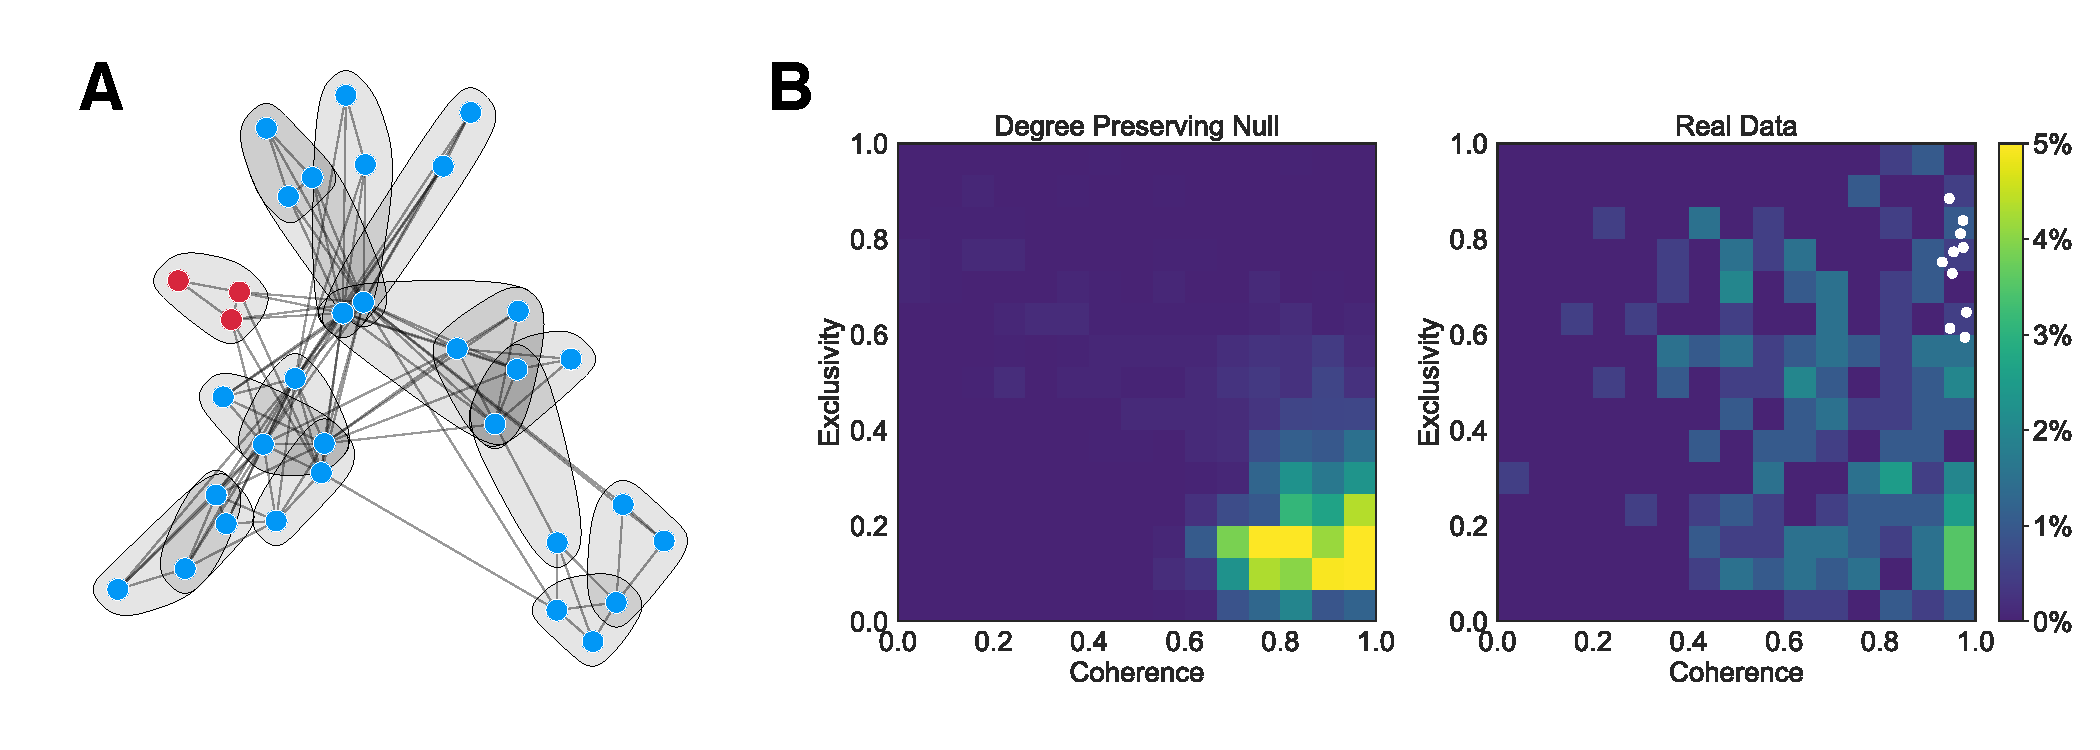
\includegraphics[width=\textwidth]{images/cartels/combined_ohio.pdf}
\caption[Ohio school milk cartel]{A. Ohio school milk market co-bidding network, 1986. Overlapping groups are detected using our algorithm. Red nodes are member of the alleged cartel operating near Cincinnati. We exclude firms participating in less than 3 auctions for the purposes of visualization. B. Coarsened two-dimensional histograms of groups detected in all Ohio school milk networks 1980-1990 in the coherence-exclusivity space. The first plot shows the distribution of the groups detected in 100 bid-degree preserving null models of each of the 10 years. The second plot shows the real distribution of groups. The cartel group's position is marked by white circles. The cartel group has both high exclusivity and coherence.}
\label{fig:ohio_overlap}
\end{figure}


\subsection{Georgian Public Procurement Markets}
We now turn to data from a much larger procurement market covering a wide range of goods and services. Specifically we collected virtually all public contracts from the Republic of Georgia from 2011 to 2016. The data consists of nearly 150,000 contracts bid on by nearly 15,000 unique firms with total value roughly five billion US dollars. As with the Ohio dataset, we observe the bids and bidder identities for each contract. We again apply our method to detect overlapping groups and calculate their coherence and exclusivity for each year. In the analysis that follows we consider only groups of firms identified from the co-bidding network that exclusively bid on at least 30 contracts in a given year in order to focus on significantly interacting firms. Our findings are robust to consider a range of cutoffs, which report in the SI.

To compare our data against a plausible null model, we created randomized networks from data by shuffling the contracts firms bid on within specific product classes. This insures that firms bidding exclusively on school milk contracts do not bid on software consulting contracts in our null model. We use the resulting distributions of group cohesion and exclusivity from the null model to create thresholds for labeling groups from the empirical network as suspicious. We consider a group from the empirical co-bidding network suspicious if its coherence and exclusivity exceed the 80th percentile of coherence and exclusivity of groups in the null model in the same year. 

We visualize the distributions of groups in the coherence and exclusivity space for the randomized and empirical data in subplot A of Figure~\ref{fig:ga_results}. We plot the data from all years in the same visualization, and highlight the suspicious zone of high coherence and exclusivity calculated for 2016.

\begin{figure}[t]
\centering
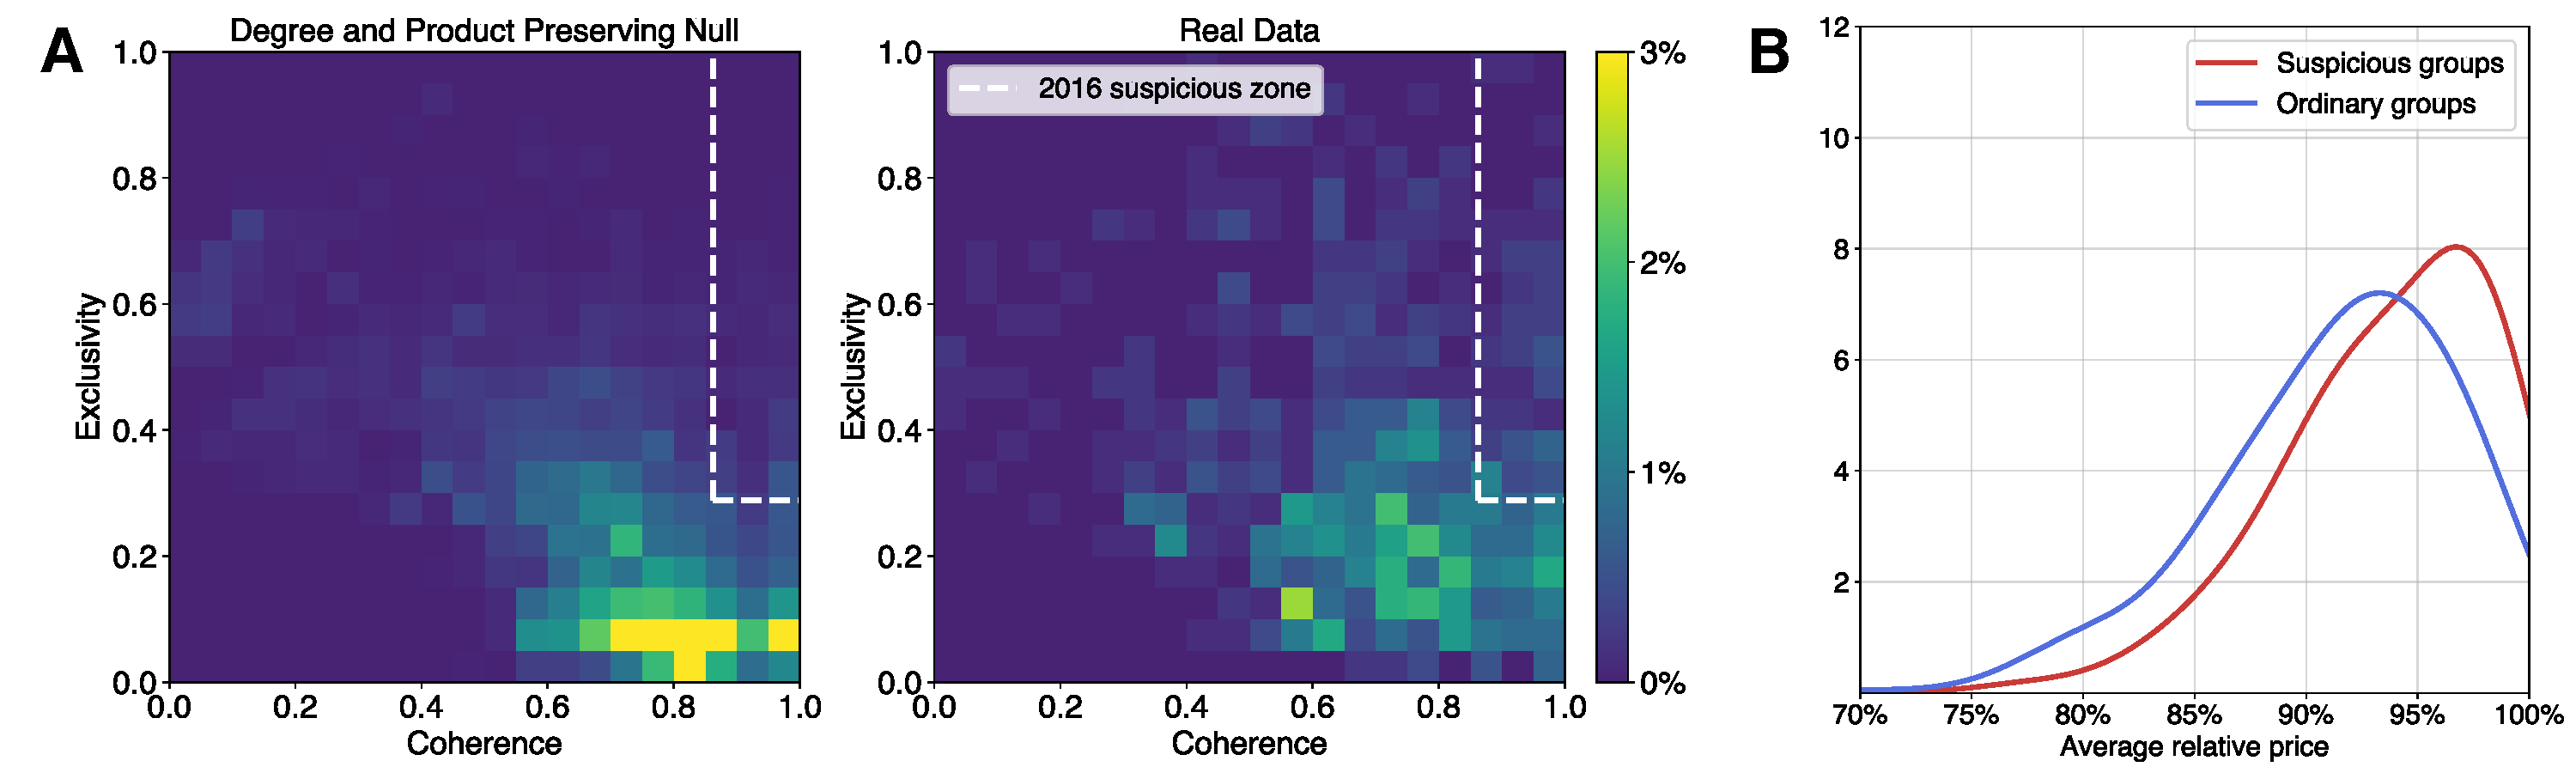
\includegraphics[width=\textwidth]{images/cartels/ga_2d_dists_and_rel_price_kdes.pdf}
\caption[Coherence and Exclusivity of Georgian groups.]{A. The distribution of groups in the cohesion-exclusivity feature space detected in a product-type and bid-degree preserving null model compared with groups detected in observed data from Georgian procurement markets from 2011-2016. We label groups of firms as suspicious if its coherence and exclusivity are in the 80th percentile of the null model outcomes of the year in which they are detected. We highlight 2016's suspicious zone in white.  B. Distribution of average relative prices of contracts bid on by suspicious groups and ordinary groups, 2011-2016. Suspicious groups consistently win more expensive contracts.}
\label{fig:ga_results}
\end{figure}

As there are no confirmed ground truth cartels in our dataset, we validate our claim that groups in the suspicious zone are operating under conditions that facilitate collusion using four measures. First we consider the average cost of contracts won by the group when they were the only participants. As contracts are announced with a reserve price, we can scale each contract's cost outcome to enable comparisons between contracts. We plot the distribution of relative prices for contracts won by suspicious groups versus all other groups in subplot B of Figure~\ref{fig:ga_results}. We confirm that groups in the suspicious zone are winning more expensive contracts, confirmed by a Mann-Whitney U test shown in Table~\ref{tab:ga_stats_table}.

Next, we calculated two price and bid based screens for collusion from the literature. The first is the price coefficient of variation of contracts won by the group~\cite{abrantes2006variance}, measuring the extent a group's prices are both high and stable. This screen is based on the theoretical observation that when prices are set collectively, it is costly to coordinate price changes~\cite{lacasse1995bid}. It aligns with empirical observations of real cartels~\cite{bolotova2008impact} and has been used extensively by competition authorities~\cite{abrantes2012lessons}. Specifically, the price coefficient of variation $CV_{price}^{G}$ of a group $G$ is defined in terms of the average cost of contracts $C$ cornered by the group, $\mu_{C}^{G}$, and the standard deviation  $\sigma_{C}^{G}$:

$$CV_{price}^{G} =\dfrac{\sigma_{C}^{G}}{\mu_{C}^{G}} $$

The second cartel screen we apply is the average of the coefficient of variation of bids on each contract for which only group firms submitted bids~\cite{imhof2017simple}. Previous research has shown that the fake bids submitted by losing members of the cartel tend to closely hug the winning bid. For each contract $c$ bid on exclusively by members of a group, we calculate the coefficient of variation in the bids:

$$CV_{bidding}^{c} =\dfrac{\sigma_{c}}{\mu_{c}} $$
We average over all contracts $C$ cornered by a group $G$ to obtain its bidding coefficient of variation:

$$CV_{bidding}^{G} =\mu_{c \in C}\left(CV_{bidding}^{c}\right) $$
We say that a group of firms has a low bidding coefficient of variation if it is less than one standard deviation below the market average. A Mann-Whitney U test, shown in Table~\ref{tab:ga_stats_table}, indicates that groups in the suspicious zone are significantly more likely to have lower $CV_{bidding}^{c}$ and $CV_{price}^{G}$. 

We carry out one more test of our method using data on bid protests. Bid protests are legal actions by firms against contracts awarded by procurement authorities. Firms can protest, for example, if the contract was not advertised in the proper venue, or if they believe criteria to participate in an auction unfairly excluded them. We collected data on which firms protested which contracts, including the firm to which the contract was awarded. We argue that colluding firms would never protest the contracts won by their cartel partners, while one may expecting intensely competing firms to frequently protest each others' winnings. For each group we check if any contract awarded to a group member was protested by another group member that year. We find that suspicious groups are half as likely to have such internal protests - a statistically significant difference shared in Table~\ref{tab:ga_stats_table}. 

\renewcommand{\tabcolsep}{2pt}
\begin{table}[]
\ra{1}
\begin{tabular}{@{}lrrrrr@{}}
& Suspicious Groups & \phantom{a}& Ordinary Groups & \phantom{a} & Differences \\
%\cmidrule{2} \cmidrule{4}  \cmidrule{6} 
&Mean (St. Dev.) &&Mean (St. Dev.) &&MW U (p-value)\\  \midrule
Avg. Rel. Price & 0.938 && 0.914&&30211^{***}  \\
&  (0.046) && (0.053) &&(p$<$0.001)  \\
Avg. $CV_{price}^{G}$ & 0.098 && 0.117&& 33470^{***}   \\
 & (0.055) && (0.059) && (p$<$0.001)  \\
Avg. $CV_{bidding}^{G}$ & 0.047 && 0.055 && 32306^{***}  \\
& (0.056) && (0.038) && (p$<$0.001)  \\
Bid Protest Rate & 0.134  && 0.237 && 37516^{*} \\
& (0.341) &&(0.425) && (p$\approx$.011)\\
\bottomrule
\end{tabular}
\caption[Cartel screen comparisons.]{Cartel screens applied to suspicious and ordinary groups of firms detected in the Georgia procurement market, 2011-2016. Cartel groups have higher average relative prices, are more likely to have a low average coefficient of variation on bids for a contract, and are less likely to legally protest the winnings of other group members. * $p < .05$, ** $p <.01$,*** $p <.001$ }
\label{tab:ga_stats_table}
\end{table}
\renewcommand{\tabcolsep}{6pt}


Suspicious groups detected by our methods are more likely to manifest the four collusive markers we have measured than their non-suspicious counterparts. Though this is no proof of collusion, it does indicate that many of the groups of firms that competition authorities might be interested in investigating based on their behavioral patterns exist in the same high coherence and exclusivity zone as the Ohio school milk cartel. In the next section we present a simple simulation model of a procurement market with spatial correlations which replicates our observation that collusion is more common among cohesive and exclusive groups.


\subsection{Simulation Model}
We simulated a market of interacting firms placed uniformly at random in the unit square. The location of firms can be interpreted as their physical location or as a more abstract position in a space of product similarities (for instance firms supplying computer hardware might be closer to one another). Contracts, also located randomly, attract bids from nearby firms, introducing spatial correlation to the interactions between firms. We assume that firms participating in an auction know the other participants. Each firm must decide whether to cooperate or compete for the contract using two factors: the firm's memory of the previous action of the other firms, and the frequency by which they have met the same firms in the recent past.

For the first factor, the focal firm recalls the previous decision made by the other firms it is meeting using a proportional tit-for-tat strategy~\cite{axelrod1981evolution}. The second factor increases the likelihood of cooperation when the other firms have been. The decision to collude depends on the product of these two: familiarity and experiences of reciprocity are essential to start and sustain collusion~\cite{hilbe2018partners}. In order to keep the model as simple as possible, we do not introduce a price mechanism or consider who wins a given auction. We seek to demonstrate that random spatial correlations can create environments with locations heterogeneously favorable to collusion. We present the precise parameters and initial conditions in the section on data and methods.

We simulated 5000 instances of our model, each time initializing a new market with randomly placed firms and contracts. In each instance we award 2,000 contracts, discarding the data from the first 1,000 contracts as burn-in. As before, we constructed the co-bidding networks of firms, detected groups in them, and plotted their distributions in Figure~\ref{fig:simulation_model}, subplot A.

For each group, we calculated the rate at which members unanimously cooperated on a contract, in other words the relatively frequency of successful collusion among the group. We plot the distribution of this frequency across the coherence-exclusivity space in subplot B. In agreement with our empirical evidence, we find that collusion is significantly more likely to emerge among groups in the region of high coherence and exclusivity.

\begin{figure}[t]
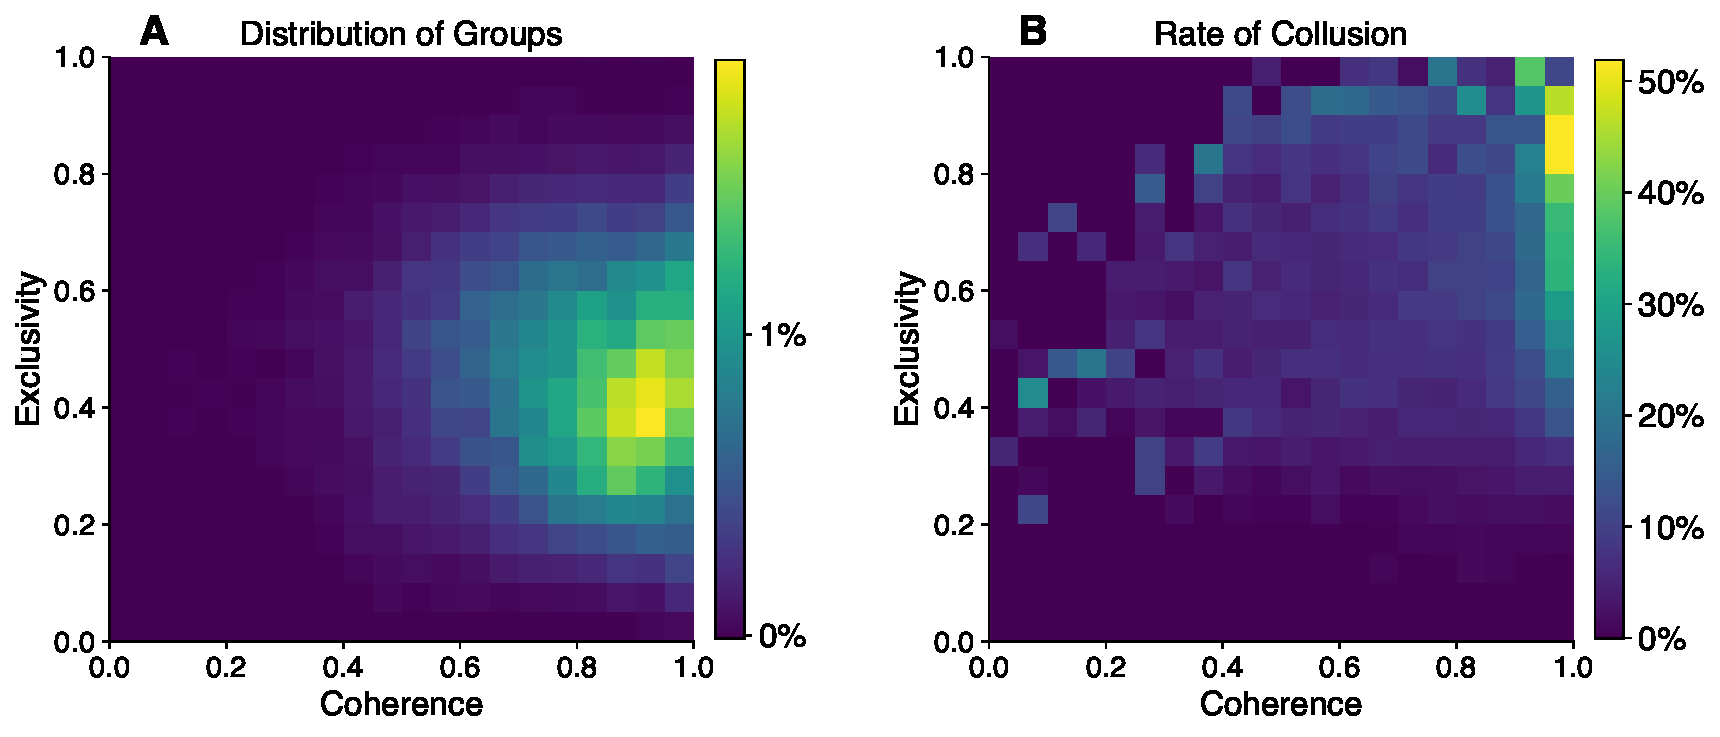
\includegraphics[width=\textwidth]{images/cartels/simulation_results.pdf}
\caption[Simulation model coherence and exclusivity distributions.]{Simulation model results over 5000 simulations. A) the distribution of groups observed from the resulting co-bidding networks in the coherence-exclusivity feature space. B) the rate of collusion by groups with given coherence-exclusivity. The model suggests that high coherence and exclusivity groups are not common, but that they have significantly higher rates of cooperation.}
\label{fig:simulation_model}
\end{figure}

As discussed earlier in the article, economic theory and empirical observation suggests that there are certain environments in which cartels are more likely to emerge~\cite{levenstein2006determines}. Inspired by the literature on evolutionary game theory, we considered a simple model of cooperation based games played between agents embedded in space~\cite{szamado2008effect}. Our findings support the notion that the co-bidding network captures localized market conditions, which in turn govern the likelihood and effectiveness of emergent cooperation. Interestingly, in the case when a market is significantly governed by the locations of firms in physical space, for example in the Ohio milk market, our model has the potential to be calibrated with geographical data.



\section{Discussion}
In this chapter we developed a framework to find groups of firms in public contracting markets and to screen them for collusive markers. Testing our method on a ground truth case, a large scale market without known collusion, and a simple model of such markets, we find that collusion seems more likely to emerge among groups of firms with cohesive and exclusive interactions. Groups occupying such distinguished places in the broader market have found a niche with conditions ripe for the emergence of cooperation.

We must acknowledge that our approach to cartel detection is only suggestive - it cannot prove that a group of firms are engaged in collusion. Rather we propose that our method be used to narrow down a large space of possibilities, into a shorter list of candidates for investigation. Authorities can then apply classical screens for evidence of illegal cooperation~\cite{harrington2006behavioral,fazekas2016}, for example by observing abnormal stability in prices or market shares~\cite{abrantes2006variance,imhof2017simple}, or by comparing observed behavior against a model of competitive behavior~\cite{bajari2003deciding,pesendorfer2000}. More granular data required for these tests for collusion can be collected once a key subset of firms is identified, at significantly lower cost. Another advantage of our approach is that it does not rely on information from whistleblowers to highlight a candidate group of firms, avoiding a potential source of bias in the cartel literature~\cite{allain2011determination}. We also acknowledge that there are other cartel strategies in public contracting markets beside bid-rigging, for instance when firms agree to stay out of each others' markets entirely.

In our model we do not consider the idea that some firms might simply be honest and refuse to form a cartel even in optimal conditions, nor do we consider how fear of prosecution might influence the choice to collude, for instance in our model. Though the illegality of collusion adds an additional obstacle to the emergence of cooperation among firms, the empirical observation that cartel life spans are heterogeneous suggests that many firms are willing to collude, but that only certain environments are conducive to cartels~\cite{levenstein2006determines}. 

In spite of the limitations, we note that our method can be applied to other questions about cartels. For example, what does the co-bidding network look like near a cartel when it is born compared to when it dies? The inner-workings of potential cartels would surely be reflected in network structure of the market. Observed cartels have operated by methods such as rotating the winner~\cite{ishii2009favor}, by side payments to losing firms~\cite{pesendorfer2000}, and some even run internal auctions to optimize their profits~\cite{asker2010study}. Observing the relationship between the procedure by which contracts are awarded, for example to the trimmed-average bidder in Italian road contracts~\cite{conley2016} or by randomly chosen open or sealed bid procedures in timber auctions~\cite{athey2011comparing}, and network structure may also reveal whether firms are competing or colluding. The specifics of a market and manner by which contracts are awarded matters a great deal to how collusion might evolve~\cite{hendricks1989}. Certain rules make it easier for firms to collude or easier to detect collusion~\cite{conley2016,athey2011comparing}. 

We are confident that our approach can be applied to these cases in which we have extra information about the rules of a market. It is likely still the case that certain patterns of interaction are effective markers of collusion and that networks provide a useful map of such interactions.


\section{Methods and Data}

\subsection{Co-bidding networks, group detection, and group features}
We define a public contracting market's \textit{co-bidding network} as a projection of a bipartite network onto the set of firms active in the market. Specifically, we form a bipartite network of contracts and firms bidding on them, then create a network of firms which bid for the same contract. We weight the connections based on the similarity of co-bidding behavior between firms using Jaccard similarity. Specifically, firm A and firm B are connected by a link with weight equal to the overlap of the contracts they bid on:

$$w_{A,B} = \dfrac{\lvert c_{A} \cap  c_{B}\rvert}{\lvert c_{A} \cup  c_{B}\rvert},$$
where $c_{A}$ ($c_{B}$) is the set of contracts of $A$ ($B$) with at least one other bidder and $|\cdot|$ is the cardinality of a set.

Given a co-bidding network our aim is to extract groups of nodes which may be analyzed for cartel activity. Groups should be communities in the network sense: there should be more interactions within the group than leaving the group. The case in question suggests several other criteria for our algorithm. Groups should be small, as cooperation becomes more difficult to sustain with more participants. Firms might be present in more than one part of the market, so we should consider overlapping groups.

We adapt a bottom-up method for community detection which merges nodes into groups by local optimization of a fitness function from previous work by Lancichinetti, Fortunato, and Kert\'esz (hence: LFK) ~\cite{lancichinetti2009detecting}. We define the fitness $f_{G}$ of a group of nodes $G$ in a network as:

$$f_{G}= \dfrac{s_{in}^{G}}
{\left(s_{in}^{G}+s_{out}^{G}\right)^{\alpha}
\times \lvert G \rvert^{\beta}},$$
where $s_{in}^{G}$ and $s_{out}^{G}$ denote the strength (the sum of weights) of edges within the group and adjacent to the group, respectively. $\lvert G \rvert$ is the size of the group, and $\alpha$ and $\beta$ are free parameters which control the size of the groups found. When $\alpha$ is increased, additional strength is penalized, while $\beta$ penalizes the number of group members independently of their strength. We set both parameters to 1.5. Increasing $\alpha$ insures that new nodes added to a group interact primarily within the group, while increasing $\beta$ restricts the size of the groups we detect, in line with the stylized facts about cartels from the economics literature that lasting cartels are small and frequently interacting~\cite{levenstein2006determines}. We report the sizes of the groups found in the empirical cases in the SI.

Given such a fitness function of a group of nodes in a co-bidding network, we can define the fitness of a node $n$ relative to a group by calculating the difference in fitness of the group with $n$ and without it:

$$f_{G}^{n}= f_{G+\{ n \}} - f_{G}$$

With this node-level measure of fitness we can define our group detection algorithm. For each node in the network:
\begin{itemize}
    \item select a node $n$ and initialize a group containing only $n$,
    \item select the neighbor of $n$ with the largest fitness and, if it has positive fitness, add it to the group. 
    \item repeat until no nodes adjacent to the group have positive fitness. 
\end{itemize}
In this way we find groups in the network which are overlapping, small (tuned by the parameters), with more weight among themselves than with non-group members. It is possible to save significant computational time by initializing new groups only for nodes that have not been included in a group before. In contrast with the LFK method we do not recalculate the individual fitness of all nodes in the group following the inclusion of a new node. In this sense our adaptation is greedy and not iterative, saving computational time.

Once groups have been extracted from a market's co-bidding network, we then define topological features of each group that may suggest that the firms could form a cartel. The first measure is the \textit{coherence}~\cite{onnela2005intensity} of a group $C_{G}$, the ratio of the geometric and arithmetic means of the edges weights among group members, measuring the balance and overall frequency of interactions among the group members:

$$C_{G}=\dfrac{\displaystyle \left(\prod_{l_{G}}w_{l}\right)^{1/\lvert l_{G}\rvert}}{\dfrac{\displaystyle \sum_{l \in G}w_{l}}{\lvert l_{G}\rvert}}$$

The second measure is \textit{exclusivity} , the ratio of strength within the group over the total strength of the group, excluding on edges to non-group members, measuring the group's relative isolation in the broader market:

$$E_{G}= \frac{s_{in}^{G}}{\left(s_{in}^{G}+s_{out}^{G}\right)}$$

\subsection{Null models}
In both empirical cases, we created null models of the market to capture the extent to which groups of certain cohesion and exclusivity emerge by chance. For the Ohio school milk data we shuffled the bidders across all contracts, preserving the number of bidders each contract received, and the number of contracts each firm bid on. In Georgia we repeated the same procedure with an additional restriction: firm bids were only shuffled among contracts with the same 2-digit Common Procurement Vocabulary (CPV) code~\cite{cpvreport}. CPV codes describe the type of good or service being contracted, from road repair to medicine. By restricting the random shuffling of bids by CPV code, we create a randomized version of the broader market which preserves the tendency of firms providing similar products to interact.

\subsection{Agent Based Model}
In this section we describe the specific parameters of our simulated model of a spatially embedded contracting market. Each simulated market was initialized with 50 firms and 75 issuers of contracts (analogous to school districts) placed uniformly at random in the unit square. We then play 2,000 rounds corresponding to contract awards.

In each round a randomly selected issuer releases a contract $C$ placed nearby (at a position drawn from a 2-d normal distribution centered on the issuer with standard deviation .3). Firms participate in the competition for the contract if they are within .1 distance of the contract (if no firms are close enough, the distance for inclusion is extended by .1 repeatedly until at least one firm participates). The set of firms participating, $F$, is known to all firms.

Each firm must then decide to collude or compete. Collusion is successful if all firms collude. Each firm $f$ considers two pieces of information about the other firms in its decision making process, its \textit{memory} of previous interactions with each other firm, and the relative \textit{frequency} with which it meets with the others. It recalls the decision made by the other firms the previous time they met (initialized randomly) and calculates the share of previous round cooperators:

$$f_{memory}=\dfrac{ \sum_{\hat{f} \in F\setminus f} 
  \delta_{\hat{f}}^{C_{prev}}}
{\|F\setminus f \|}, $$

where $\delta_{\hat{f}}^{C_{prev}}$ equal 1 if $\hat{f}$ cooperated the last time it encountered $f$. This is the proportional (compared to the absolute) generalization of the tit-for-tat strategy to multi-agent games~\cite{axelrod1981evolution}.

Next, $f$ considers how often, in the last $k$ contracts it was participating in, the current other firms were a subset of the participating firms. If this is true at least two-thirds of the time, the firm considers the other firms it meets as familiar.

$$ f_{frequency} = 
    \begin{cases}
      1, & \text{if}\ \dfrac{\sum_{i=1}^{k} \delta_{F \subset F(C_{f}^{i})}}{k} \geq 2/3 \\
      0, & \text{otherwise}
    \end{cases}
$$

where $F(C_{f}^{i})$ denotes the firms participating in the $i$'th previous contract of firm $f$. $f_{frequency}$ increases as $f$ tends to meet the same firms. We set $k$ to 10. 

The focal firm's decision to collude or compete depends on the product of these two factors:

$$f_{compete} =  
    \begin{cases}
      1, & \text{if}\ f_{memory} * f_{frequency} \geq .9 \\
      0, & \text{otherwise}
    \end{cases}
$$

Finally, we add noise to the system by allowing a .1\% chance that a firm spontaneously colludes. In our model agents do not learn or track the outcome of their actions - they only react to their most recent memory of other firms and the frequency by which they meet. After 2,000 contracts are awarded, we end the simulation and discard the outcomes of the first 1,000 contracts as burn-in.



\subsection{Datasets}
The Ohio school milk data was generously provided by Porter and Zona~\cite{porter1999ohio}. The data consists of a significant share of all school-milk procurement contracts from 1980s Ohio provided to Porter and Zona by the State of Ohio. Porter and Zona served as expert witnesses in a trial against the suspect cartel. There are several other significant examples of cartels in public school milk markets in the US during the 1980s, for example in Florida and Texas~\cite{pesendorfer2000,hewitt1993incumbency}.

We collected the Georgian contracts dataset from the centralized procurement portal of the State Procurement Agency (SPA) of Georgia\footnote{https://tenders.procurement.gov.ge/}, including all contracts awarded through the portal between 2011 and 2016. Contracts are awarded to the lowest bidder in a sealed-bid auction. Each contract includes a product category (CPV code~\cite{cpvreport}, which we use for the null model, and a reserve price, the maximum price that the public buyer would pay for the good or service, which we use to normalize prices. The procurement portal also reports bid protests: these are legal disputes of participants in the procurement process against the agency issuing a contract. For example, a firm may protest that it was unfairly excluded from the competition for a contract.

\pagestyle{fancy} %Bike algorithms
%\chapter{Conclusion}

This thesis set out to demonstrate the utility of a network perspective on corruption. Noting that previous approaches to the study of corruption are either often overly atomic or overly structural, we framed corruption as an emergent phenomenon occurring between actors within the networks of their interactions. We leveraged the recent proliferation of data on public procurement to create transaction-level measures of corruption risk, which we embed in social and economic contexts. Our approach is validated by the observation that bad behavior at the dyadic level (i.e. between a corruption issuer and winner or among colluding firms) is related to and to some extent predicted by the network the dyad is embedded in~\cite{granovetter1985economic}.

We have seen that social networks in a place relate to the prevalence of corruption in its local government. The findings of Chapter 3 suggest that certain modes of social organization facilitate corrupt behavior. These modes are increasingly observable and measurable at the level of societies because of the vast amount of data created by the use of modern telecommunication services. This suggests why corruption is a stubborn phenomenon, and why most interventions don't work.

At the national level, we saw in Chapter 4 that corruption risk is distributed in very different ways across EU countries, nearly independent of the overall level of corruption risk observed in a country. In some countries with high levels of corruption risk, corruption is significantly concentrated in the relationships between core issuers and winners, while in other countries corruption is more concentrated among peripheral actors. Corruption risk tends to cluster in all countries in our analysis, though the extent to which it does varies greatly. Finally, we also observe significant heterogeneity in the response of corrupt relationships to political shocks. These differences have significant implications for anti-corruption strategies, casting doubt on global solutions. Indeed one could say that while countries with little amounts of corruption are similar, each highly corrupt country is corrupt in its own way.

Finally, we presented a method to detect potential hot-spots for the emergence of illegal collusion in competitive markets using data on bidding. Using two empirical cases and a simulated model we showed how groups occupying specific positions in the co-bidding network topology are uniquely able to sustain the cooperation needed to maintain a cartel. Our framework demonstrates a way to reduce the vast complexity of a market to highlight groups of firms worth investigating.  

Given previous work on the networked nature of criminal conspiracies, it is perhaps no surprise that a study of corruption and collusion in procurement markets found significant relationships between network structure and bad behavior. We argue that the specific methods developed and analyses carried out offer actionable insights into how corruption works in different contexts. They also offer a kind of blueprint for future analyses, showing how procurement data can be analyzed using network methods.

\subsection*{Future Work}
The future for data-driven anti-corruption research looks bright. Data quality and access are generally improving. New sources of data will go a long way to addressing some of the shortcomings and limitations of the work in this thesis. For example, data on company owners and board members and the economic and social relations of politicians and regulators have potential to extend the scope of the work presented in this thesis. Network methods are clearly applicable in these contexts as well. For instance, by tracking social network connections of firm leaders to people in power, one could measure the extent of political corruption in a country by the effect of such connections on profitability.

A major challenge in corruption research using big data will be to carry out causal inference. Though data collected at large scales has many advantages, for instance allowing us to observe whole markets across significant periods of time, it seems unrealistic to carry out experimental studies at the same scale, especially without the participation of government bodies. Further research is needed to extend methods of causal inference, for instance as often applied to panel data by economists, to the setting of networks.

In the absence of causal identification, the scientific value of the methods developed in this thesis can be tested in other ways. If network analyses of procurement based risk indicators can predict corruption cases that authorities, researchers, or journalists can confirm, that would lend additional credibility to our approach. One can also strengthen the validity of these methods by finding evidence of other kinds of white-collar crime occurring among distinguished actors, following the classical adage that ``where there is smoke, there is fire''.

The involvement of governments in anti-corruption research presents both opportunities and dangers. Public actors willing to experiment with rules or enforcement can help overcome problems of causal interpretation inherent in the study of observational data. Such collaborations also have the greatest potential for real-world impact, clearly. However, if researchers of corruption focus their attention too much on such collaborations, they would introduce a significant bias to our understanding of corruption. Indeed, where corruption is endemic, it is unlikely that relevant government bodies would be willing to participate in effective anti-corruption studies. Engagement with super-national actors with some independent authority in certain locations, for example with the World Bank in its procurement-based development projects or the EU and it cohesion funds, would overcome this issue to some extent. Certainly, the first step in this direction would be to convince individuals in these organizations of the value of network methods in the study of corruption. We hope that this thesis will be useful in this regard. 

\pagestyle{fancy} 

\bibliographystyle{bmc-mathphys}
\bibliography{bibliography.bib}


%\chapter{Appendices}

\section{Life quality as walkability}

\subsection{Secondary data sources}
\label{SI:walkabilityData}
\begin{itemize}
  \item {Sport associations in Budapest}~\cite{HU_sport}
  \item {Kindergartens, daycares, primary and secondary education}~\cite{HU_Edu}
  \item {Art and music schools}~\cite{HU_Art}
  \item {Child health services}~\cite{HU_Child}
  \item {Social welfare system (eg.: elderly care)}~\cite{HU_Social}
  \item{Culture centers}~\cite{HU_Cult}
  \item {Indoor playgrounds}~\cite{HU_Play}
  \item{Healthcare (hospitals, private and public clinics, specialists)}~\cite{HU_Health}
  \item{Fitness and training facilities}~\cite{HU_Fitness}
  \item{Outdoor fitness facilities}~\cite{HU_outfitness}
  \item{Thermal baths and spa}~\cite{HU_Thermal}
  \item{Playgrounds and parks}~\cite{HU_Park}
\end{itemize}

\section{Weights used in the calculations}
The weights of the different $Q$ indices in the final aggregation as well as in sub-categories highly depends on the context and the nature of the problem. Here we present the values we used to generate the results of this study, that were agreed upon consulting with experts.\\
The weights of the sub-indices from equation (\ref{final_Q}) are of the following values:\\
$w^{services}=0.7$\\
$w^{safety}=0.1$\\
$w^{environment}=0.2$\\ \\
The category weights used in equation (\ref{Q_services}), aggregating $Q^{services}$ are:\\
$w^{family}= 0.3$;\\
$w^{health}= 0.3$;\\
$w^{culture} = 0.15$;\\
$w^{sport} = 0.15$;\\
$w^{night life}=0.1$;\\\pagestyle{fancy}
%\newpage
\backmatter
\afterpage{\blankpage}
\end{document}
